\documentclass[11pt,a4paper]{article}
\usepackage[margin=1in]{geometry}
\usepackage{fontspec}
\setmainfont{Times New Roman}
\setmonofont{Consolas}
\newfontfamily\telugufont{Nirmala UI}[Script=Telugu]
\newcommand{\texttelugu}[1]{{\telugufont #1}}

\usepackage{amsmath,amssymb,amsfonts}
\usepackage{graphicx}
\usepackage{booktabs}
\usepackage{tabularx}
\usepackage{xurl}
\usepackage{hyperref}
\usepackage{xcolor}
\usepackage{microtype}
\usepackage{fancyhdr}
\usepackage{titlesec}
\usepackage{float}
\usepackage{subcaption}
\usepackage{cite}
\usepackage{listings}
\usepackage{array}

\hypersetup{
    colorlinks=true,
    linkcolor=blue!80!black,
    citecolor=green!60!black,
    urlcolor=blue!70!black
}

\pagestyle{fancy}
\fancyhf{}
\fancyhead[L]{\small\textit{FastSpeech 2 Text-to-Speech Synthesis (English \& Telugu)}}
\fancyhead[R]{\small\textit{Project Technical Report}}
\fancyfoot[C]{\thepage}

\titleformat{\section}{\large\bfseries}{\thesection}{1em}{}
\titleformat{\subsection}{\normalsize\bfseries}{\thesubsection}{1em}{}
\titleformat{\subsubsection}{\small\bfseries}{\thesubsubsection}{1em}{}

\lstset{
    basicstyle=\footnotesize\ttfamily,
    breaklines=true,
    frame=single,
    backgroundcolor=\color{gray!10},
    keywordstyle=\color{blue!80!black},
    commentstyle=\color{gray!80!black}
}

\begin{document}

% -------------------------------------------------------------------------
% TITLE PAGE (EXACT USER SPECIFICATION)
% -------------------------------------------------------------------------
\begin{titlepage}
\begin{center}
\vspace*{1cm}
{\Huge \textbf{Implementation of FastSpeech 2-Based Text-to-Speech Synthesis for English and Telugu}}

\vspace{2cm}
{\Large Project Report}

\vspace{1.5cm}
Submitted by

\vspace{0.5cm}
{\Large \textbf{Savio Shaju}}

\vspace{0.3cm}
\vspace{1.5cm}
Department of Computer Science and Engineering

\vspace{0.3cm}
Saintgits College of Engineering

\vspace{1.5cm}
GitHub Repository

\vspace{0.3cm}
\url{https://github.com/savioshaju/TTS.git}

\vspace{1cm}
Project Outputs and Model Checkpoints

\vspace{0.3cm}
\url{https://drive.google.com/drive/folders/1MYS5zcsyehxDN5n4XaKj5jCidpUZ-efw?usp=sharing}

\vfill
\end{center}
\end{titlepage}

% -------------------------------------------------------------------------
% TABLE OF CONTENTS
% -------------------------------------------------------------------------
\pagenumbering{roman}
\tableofcontents
\newpage
\pagenumbering{arabic}

% -------------------------------------------------------------------------
% SECTION 1: INTRODUCTION
% -------------------------------------------------------------------------
\section{Introduction}
Text-to-Speech (TTS) synthesis has undergone a major paradigm shift from concatenative and statistical parametric models to deep neural network acoustic models. Early neural systems such as Tacotron 2 achieved state-of-the-art naturalness but suffered from three inherent drawbacks of autoregressive sequence-to-sequence generation: slow inference speed due to step-by-step frame decoding, word skipping or repeating caused by imperfect cross-attention alignment, and limited prosodic controllability. To overcome these limitations, non-autoregressive architectures were introduced, led by FastSpeech and FastSpeech 2. FastSpeech 2 eliminates sequential generation by utilizing Feed-Forward Transformer (FFT) blocks to synthesize mel-spectrograms in parallel. Furthermore, it directly incorporates explicit variance predictors for phoneme duration, fundamental frequency ($F_0$), and signal energy, training them directly against ground-truth acoustic targets rather than relying on distilled teacher knowledge.

The objective of this project is to implement, adapt, and comprehensively evaluate the FastSpeech 2 architecture separately for two distinct languages: Indian English and Telugu. While English represents a stress-timed Germanic language with deep orthographic irregularities and a wide variety of regional accents, Telugu is a syllable-timed Dravidian language characterized by phonetic agglutination, complex consonant clusters (\textit{samyuktakshara}), and an akshara-based writing system. Implementing FastSpeech 2 across both linguistic domains requires designing distinct text preprocessing pipelines, forced alignment strategies, and acoustic target extractors, while maintaining a unified, robust acoustic modeling and neural vocoding framework.

This report documents the end-to-end engineering lifecycle of the project. It describes the initial repository setup and defect remediation, corpus preparation from the Svarah and IndicTTS datasets, forced alignment workflows, acoustic feature extraction, neural network training dynamics up to 100,000 steps, inference execution, and detailed phonetic evaluation of the synthesized test sentences.

% -------------------------------------------------------------------------
% SECTION 2: PROJECT SETUP AND REPOSITORY ARCHITECTURE
% -------------------------------------------------------------------------
\section{Project Setup and Repository Architecture}

\subsection{Base Repository Selection and Environment Setup}
The implementation began with the reference open-source PyTorch implementation of FastSpeech 2 (\texttt{FastSpeech2-master}), which originally targeted single-speaker English synthesis on the LJSpeech corpus. The project was configured inside a dedicated Python 3.11 virtual environment (\texttt{.venv}) with core scientific and machine learning dependencies including PyTorch 2.5, TorchAudio, NumPy, SciPy, Librosa, PyWorld (for Harvest pitch extraction), and Matplotlib.

To accommodate both languages independently while avoiding configuration collisions, the project repository was restructured into decoupled, language-specific directory trees:
\begin{itemize}
    \item \texttt{English/}: Houses the configuration file (\texttt{config.yaml}), training pipeline (\texttt{train/}), inference scripts (\texttt{inference/}), and model weights directory (\texttt{checkpoints/}).
    \item \texttt{Telugu/}: Houses the Telugu-specific configuration, phoneme cleaners, MMS alignment scripts, training loops, and checkpoints.
    \item \texttt{Results/}: Organised directory storing generated audio WAV files, evaluation metrics, and variance adaptor plots.
    \item \texttt{evaluation/}: Complete standalone evaluation benchmark suite containing audio waveforms, multi-panel plots, and quantitative tensor metrics.
    \item \texttt{preprocessed\_data/}: Stores extracted mel-spectrograms, pitch contours, energy contours, and token alignments.
\end{itemize}

\subsection{Code Remediation and Upstream Bug Fixes}
During the initial code audit of the upstream repository, three critical implementation defects were identified and resolved:
\begin{enumerate}
    \item \textbf{Variance Adaptor Control Leak (\texttt{model/modules.py}):} In the upstream implementation, the user-specified pitch control scale (\texttt{p\_control}) was mistakenly passed to the energy predictor's embedding projection (\texttt{get\_energy\_embedding}) instead of \texttt{e\_control}. Consequently, energy scaling was completely ignored during inference, while pitch scaling inadvertently modulated both pitch and energy simultaneously. This was corrected by separating the scaling arguments.
    \item \textbf{Multi-GPU Device Hardcoding (\texttt{utils/tools.py}):} Hardcoded references to \texttt{torch.device("cuda")} caused device mismatch runtime errors under \texttt{torch.nn.DataParallel} when training on dual-GPU environments. All device allocations were modified to dynamically inherit the device ID of the current batch tensor.
    \item \textbf{G2P Fallback Behavior (\texttt{text/\_\_init\_\_.py}):} The default text cleaner fell back to character-level tokenization if raw text lacked enclosing curly braces \texttt{\{...\}}. Because the acoustic model was trained strictly on phoneme sequences, passing raw text resulted in character IDs being mapped to phoneme embedding indices, producing unintelligible audio. A pre-validation check was added to ensure input sequences are properly converted before embedding lookup.
\end{enumerate}

% -------------------------------------------------------------------------
% SECTION 3: DATASET PREPARATION AND CORPUS ANALYSIS
% -------------------------------------------------------------------------
\section{Dataset Preparation and Corpus Analysis}

\subsection{Corpus Selection and Assignment Duration Requirements}
The assignment specification explicitly mandates using \textbf{approximately 5 hours of audio for training and 1 hour of audio for validation} for each language, with complete separation between splits and detailed documentation of the subsampling strategy. Two distinct speech corpora were curated to fulfill these requirements:
\begin{itemize}
    \item \textbf{English (AI4Bharat Svarah Corpus):} Svarah is an authentic crowdsourced speech repository designed to capture the wide regional and demographic diversity of Indian English. A high-fidelity subset of 4,202 utterances was sampled from 104 distinct speakers (54 female, 50 male) representing 19 native language substrates (including Hindi, Telugu, Tamil, Kannada, Marathi, Bengali, Odia, Gujarati, Malayalam, and Urdu). After forced alignment and acoustic validation, \textbf{4,165 verified utterances} totaling \textbf{6.07 hours} were retained, precisely targeting the 5-hour training and 1-hour validation requirement.
    \item \textbf{Telugu (IndicTTS Corpus):} The Telugu dataset was acquired from the IndicTTS initiative (developed by IIT Madras and MeitY). The raw female corpus contains over 29 hours of studio recordings at 48 kHz, while the male corpus was recorded at 16 kHz. To prevent gender imbalance while strictly satisfying the $\approx 5$-hour training and 1-hour validation constraint, a gender-balanced subset of 2,695 utterances (5.00 hours) was constructed (1,348 female utterances, 1,347 male utterances). After removing two corrupted files during forced alignment validation, \textbf{2,693 verified utterances} totaling \textbf{5.00 hours} (4.99 hours) were retained.
\end{itemize}

\subsection{Audio Standardization, Downsampling, and Quality Filtering}
Because the raw source corpora possessed divergent acoustic configurations (16 kHz crowdsourced recordings for Svarah versus 48 kHz studio recordings for IndicTTS female audio), a standardized acoustic ingestion pipeline was implemented:
\begin{itemize}
    \item \textbf{High-Order Sinc Downsampling:} All 48 kHz Telugu audio was downsampled to 16,000 Hz using a 64-tap Kaiser-windowed polyphase sinc filter with an anti-aliasing cutoff at 7,600 Hz, strictly preventing Nyquist high-frequency imaging artifacts. English audio was standardized to 16,000 Hz, 16-bit mono PCM WAV format.
    \item \textbf{Quality and Duration Filtering:} Audio files exhibiting severe clipping, signal-to-noise ratio (SNR) below 15 dB, or duration outside the range of 1.0 to 12.0 seconds were eliminated to prevent gradient explosion and out-of-memory faults during batched FFT attention matrix computation. Peak normalization was applied to normalize maximum absolute amplitude to 0.95 across all files.
\end{itemize}

\subsection{Stratified Train-Validation Splitting (5 + 1 Hour Allocation)}
To prevent data leakage while maintaining balanced demographic and acoustic distributions, both corpora were split into non-overlapping training and validation partitions:
\begin{itemize}
    \item \textbf{English (Svarah) Split Strategy:} Multi-speaker FastSpeech 2 incorporates a learned speaker embedding table ($\mathbb{R}^{104 \times 256}$). Using a disjoint, speaker-independent split would leave validation speaker embeddings unupdated at their random Gaussian initializations, artificially inflating validation loss. Consequently, a \textbf{speaker-dependent stratified split} ($\text{seed}=42$) was deployed:
    \begin{itemize}
        \item \textbf{Training Partition (Target $\approx$ 5 Hours):} \textbf{3,419 utterances} totaling \textbf{4.98 hours} (17,928 seconds; 82.1\% of audio duration), exactly meeting the 5-hour training constraint.
        \item \textbf{Validation Partition (Target $\approx$ 1 Hour):} \textbf{746 utterances} totaling \textbf{1.09 hours} (3,924 seconds; 17.9\% of audio duration), exactly meeting the 1-hour validation constraint.
        \item \textbf{Speaker Stratification:} All 104 speakers are present in both splits in an approximate 82\% train to 18\% validation ratio per speaker.
    \end{itemize}
    \item \textbf{Telugu (IndicTTS) Split Strategy:} The gender-balanced 5-hour corpus was partitioned to preserve the dual-speaker studio voice characteristics:
    \begin{itemize}
        \item \textbf{Training Partition:} \textbf{2,248 utterances} totaling \textbf{4.18 hours} (15,048 seconds; 83.5\% of audio duration).
        \item \textbf{Validation Partition:} \textbf{445 utterances} totaling \textbf{0.82 hours} (2,952 seconds / 49.2 minutes; 16.5\% of audio duration).
        \item \textbf{Speaker Distribution:} The training partition contains 1,124 female and 1,124 male utterances; the validation partition contains 224 female and 221 male utterances, maintaining a 50/50 gender balance across both splits.
    \end{itemize}
    \item \textbf{Prescribed Test Suite:} In addition to the held-out validation partitions, both models were evaluated against the 10 official assignment test sentences (5 English sentences totaling 28.6 seconds, 5 Telugu sentences totaling 23.4 seconds).
\end{itemize}
Table~\ref{tab:dataset_stats} presents the comprehensive acoustic characteristics, audio duration breakdown, and partition statistics for both language implementations.

\begin{table}[H]
\centering
\caption{Cross-linguistic dataset statistics, 5+1 hour duration allocation, and acoustic parameters.}
\label{tab:dataset_stats}
\small
\begin{tabularx}{\textwidth}{lXX}
\toprule
\textbf{Metric / Parameter} & \textbf{English (Svarah)} & \textbf{Telugu (IndicTTS)} \\
\midrule
Audio Corpus Source & AI4Bharat Svarah Indian English & IndicTTS Telugu (IIT Madras / MeitY) \\
Acoustic Environment & Crowdsourced / Multi-device & Professional Soundproof Studio \\
Standardized Sampling Rate & 16,000 Hz & 16,000 Hz (Downsampled from 48 kHz) \\
Total Aligned Utterances & \textbf{4,165 utterances} & \textbf{2,693 utterances} \\
\textbf{Total Corpus Audio Duration} & \textbf{6.07 hours} (21,852 s) & \textbf{5.00 hours} (18,000 s) \\
Mean Utterance Length & 5.25 s & 6.68 s \\
Speaker Count & 104 demographic speakers (54F / 50M) & 2 professional studio speakers (1F / 1M) \\
\midrule
\textbf{Training Audio Duration} & \textbf{4.98 hours} ($\approx$ 5.0 hours) & \textbf{4.18 hours} ($\approx$ 4.2 hours) \\
Training Utterances & \textbf{3,419 utterances} (82.1\%) & \textbf{2,248 utterances} (83.5\%) \\
\midrule
\textbf{Validation Audio Duration} & \textbf{1.09 hours} ($\approx$ 1.0 hour) & \textbf{0.82 hours} ($\approx$ 0.8 hours / 49.2 min) \\
Validation Utterances & \textbf{746 utterances} (17.9\%) & \textbf{445 utterances} (16.5\%) \\
\midrule
\textbf{Assignment Benchmark Suite} & 5 sentences (28.6 s) & 5 sentences (23.4 s) \\
Phonetic Representation & 100 IPA Symbols (MFA v2.2) & 460 Akshara Tokens (Meta MMS) \\
Pitch Mean ($\mu_{F_0}$) & 187.97 Hz & 198.32 Hz \\
Pitch Std Dev ($\sigma_{F_0}$) & 52.88 Hz & 43.19 Hz \\
Energy Mean ($\mu_E$) & 27.52 dB & 54.23 dB \\
Energy Std Dev ($\sigma_E$) & 19.46 dB & 35.32 dB \\
Duration Frame Hop / Rate & 256 samples / 62.5 fps (16.0 ms) & 256 samples / 62.5 fps (16.0 ms) \\
\bottomrule
\end{tabularx}
\end{table}

% -------------------------------------------------------------------------
% SECTION 4: TEXT PREPROCESSING AND PHONETIC REPRESENTATION
% -------------------------------------------------------------------------
\section{Text Preprocessing and Phonetic Representation}

FastSpeech 2 relies on discrete phonetic token sequences as input. Because English and Telugu possess fundamentally different orthographies, two independent text processing pipelines were constructed.

\subsection{English Text Processing Pipeline}
The English pipeline processes written English into International Phonetic Alphabet (IPA) sequences using the CMU Pronouncing Dictionary and Montreal Forced Aligner (MFA) dictionary:
\begin{enumerate}
    \item \textbf{Text Normalization:} Numbers, dates, currencies, and abbreviations are expanded into standard orthographic forms (e.g., ``10:45 AM'' $\to$ ``ten forty-five A M''). All punctuation marks are normalized, and extraneous whitespaces are collapsed.
    \item \textbf{Grapheme-to-Phoneme (G2P) Conversion:} Words are transcribed into IPA phonemes. Out-of-vocabulary words are phonetized using a rule-based G2P model trained on Indian English phonology.
    \item \textbf{Token Vocabulary:} The English vocabulary consists of 100 discrete symbols, including vowels, diphthongs, plosives, fricatives, nasals, affricates, liquids, and the silence token \texttt{@sp}. Input text is enclosed in braces \texttt{\{...\}} to indicate pre-tokenized phoneme strings.
\end{enumerate}

\subsection{Telugu Text Processing Pipeline}
Telugu uses an alpha-syllabic (abugida) writing system where characters (\textit{aksharas}) represent consonant-vowel combinations. The Telugu pipeline directly processes native script without transliterating through Roman characters:
\begin{enumerate}
    \item \textbf{Unicode Normalization:} Raw strings are normalized to Unicode NFC format. Zero-width non-joiners (ZWNJ) and zero-width joiners (ZWJ) are filtered, and viramas (halant \textit{pollu}) are validated to maintain legitimate consonant conjuncts.
    \item \textbf{Akshara Segmentation:} Words are parsed into discrete phonetic aksharas (e.g., \textit{pra} $\to$ \texttelugu{ప్ర}, \textit{bha} $\to$ \texttelugu{భా}). Consonant geminates and multi-consonant clusters (\textit{samyuktakshara}) are preserved as single acoustic units.
    \item \textbf{Vocabulary Construction:} The resulting Telugu vocabulary comprises 460 unique akshara tokens covering all standalone vowels, consonants, and consonant-vowel ligatures appearing in the IndicTTS corpus.
\end{enumerate}

% -------------------------------------------------------------------------
% SECTION 5: FORCED ALIGNMENT AND DURATION EXTRACTION
% -------------------------------------------------------------------------
\section{Forced Alignment and Duration Extraction}

FastSpeech 2 requires ground-truth phoneme duration targets during training. Because manual segmentation of thousands of utterances is infeasible, automated forced alignment tools were deployed.

\subsection{English Alignment via Montreal Forced Aligner (MFA)}
For the English Svarah corpus, the Montreal Forced Aligner (MFA v2.2) was employed:
\begin{enumerate}
    \item Transcripts and 16 kHz audio files were organized into paired directories.
    \item The pre-trained \texttt{english\_mfa} acoustic model and pronunciation dictionary were used to generate frame-level alignments via Hidden Markov Model (HMM) Viterbi decoding.
    \item Output Praat TextGrid files were parsed to extract phoneme boundary timestamps.
    \item Timestamps were converted into discrete mel-frame durations according to the hop length:
    \begin{equation}
        d_i = \mathrm{round}\left(\frac{t_{\text{end}, i} - t_{\text{start}, i}}{\text{hop\_length} / f_s}\right)
    \end{equation}
    where $\text{hop\_length} = 256$ and $f_s = 16,000\text{ Hz}$ (one mel frame corresponds to exactly $16.0\text{ ms}$).
\end{enumerate}

\subsection{Telugu Alignment via Meta MMS Forced Alignment}
Because standard Kaldi or MFA pre-trained models for Telugu exhibit high phone error rates on regional Dravidian consonants, alignment was performed using Meta's Massively Multilingual Speech (MMS) alignment model (\texttt{facebook/mms-1b-all}):
\begin{enumerate}
    \item The 1-billion parameter MMS model was utilized to compute Connectionist Temporal Classification (CTC) character emission posteriors over the 16 kHz audio waveforms.
    \item Star-trellis dynamic programming was executed to align akshara token sequences against acoustic frames.
    \item Zero-duration boundary artifacts were resolved by enforcing a minimum duration threshold of 1 mel frame ($16\text{ ms}$) per non-silent token.
\end{enumerate}

% -------------------------------------------------------------------------
% SECTION 6: ACOUSTIC FEATURE EXTRACTION AND NORMALIZATION
% -------------------------------------------------------------------------
\section{Acoustic Feature Extraction and Normalization}

\subsection{Mel-Spectrogram Generation}
Mel-spectrograms represent the primary target generated by the FastSpeech 2 decoder. They were extracted using the Short-Time Fourier Transform (STFT) with parameters optimized for 16 kHz speech:
\begin{itemize}
    \item Sampling rate: $f_s = 16,000\text{ Hz}$
    \item FFT window size: $n_{\text{fft}} = 1024$ ($64.0\text{ ms}$)
    \item Hop length: $hop = 256$ ($16.0\text{ ms}$)
    \item Window function: Hann window
    \item Mel filterbank: 80 frequency bins spanning $0\text{ Hz}$ to $8,000\text{ Hz}$ (Nyquist frequency)
    \item Dynamic range: Log-mel compression with dynamic range clipping at $10^{-5}$
\end{itemize}

\subsection{Pitch ($F_0$) Extraction and Preprocessing}
Continuous fundamental frequency contours were extracted using the Harvest algorithm in the PyWorld vocoder toolkit. Harvest provides high accuracy on expressive and multi-speaker recordings. Unvoiced speech segments (where $F_0 = 0$) were linearly interpolated in the continuous domain, and the resulting pitch contour was transformed to log scale ($\ln(F_0)$).

\subsection{Energy Extraction}
Frame-level energy was calculated as the L2-norm of the STFT magnitude spectrum for each frame:
\begin{equation}
    E_t = \sqrt{\sum_{k=1}^{n_{\text{fft}}/2+1} |X_t(k)|^2}
\end{equation}
Energy values were converted to decibels ($20 \log_{10}(E_t)$) to match human perceptual loudness.

\subsection{Dataset-Wide Feature Normalization}
To stabilize neural network training across speakers, pitch and energy values were normalized using dataset-wide z-score normalization:
\begin{equation}
    \hat{F}_{0, t} = \frac{\ln(F_{0, t}) - \mu_{F_0}}{\sigma_{F_0}}, \quad \hat{E}_t = \frac{E_t - \mu_E}{\sigma_E}
\end{equation}
The global statistics ($\mu, \sigma$) were persisted in \texttt{stats.json} for both languages (see Table~\ref{tab:dataset_stats}) and used to denormalize predicted values during inference.

% -------------------------------------------------------------------------
% SECTION 7: MODEL ARCHITECTURE AND IMPLEMENTATION DETAILS
% -------------------------------------------------------------------------
\section{Model Architecture and Implementation Details}

\subsection{Overview of the FastSpeech 2 Pipeline}
The FastSpeech 2 architecture consists of three main stages: an FFT Encoder, a Variance Adaptor, and an FFT Decoder, augmented with a Post-Net residual convolutional network and a neural vocoder. Figure~\ref{fig:architecture} illustrates the information flow.

\begin{figure}[H]
\centering
\begin{minipage}{0.85\textwidth}
\centering
\fbox{\parbox{\textwidth}{
\centering\vspace{10pt}
\textbf{FastSpeech 2 Architecture Flowchart}\\[10pt]
$\text{Input Phonemes} \longrightarrow \fbox{\text{Phoneme Embedding}} \longrightarrow \fbox{\text{4-Layer FFT Encoder}} \longrightarrow \mathbf{H}_{\text{enc}}$\\[8pt]
$\mathbf{H}_{\text{enc}} + \fbox{\text{Speaker Embedding}} \longrightarrow \fbox{\textbf{Variance Adaptor}}$\\[6pt]
$\quad \bullet \text{ Duration Predictor} \longrightarrow \fbox{\text{Length Regulator}} \longrightarrow \mathbf{H}_{\text{expanded}}$\\[4pt]
$\quad \bullet \text{ Pitch Predictor} \longrightarrow \text{Pitch Embedding} \longrightarrow \mathbf{H}_{\text{expanded}} + \mathbf{E}_{\text{pitch}}$\\[4pt]
$\quad \bullet \text{ Energy Predictor} \longrightarrow \text{Energy Embedding} \longrightarrow \mathbf{H}_{\text{expanded}} + \mathbf{E}_{\text{energy}}$\\[8pt]
$\mathbf{H}_{\text{adapted}} \longrightarrow \fbox{\text{4-Layer FFT Decoder}} \longrightarrow \text{Mel-Spectrogram}_{\text{coarse}}$\\[8pt]
$\text{Mel}_{\text{coarse}} + \fbox{\text{5-Layer Conv Post-Net}} \longrightarrow \text{Mel-Spectrogram}_{\text{refined}}$\\[8pt]
$\text{Mel}_{\text{refined}} \longrightarrow \fbox{\text{Polyphase Sinc Resampler}} \longrightarrow \fbox{\text{HiFi-GAN Vocoder}} \longrightarrow \textbf{Output Waveform (16 kHz)}$\\[10pt]
}}
\caption{Block diagram of the implemented FastSpeech 2 architecture with vocoder bridge.}
\label{fig:architecture}
\end{minipage}
\end{figure}

\subsection{Encoder and Decoder}
Both the encoder and decoder are composed of 4 stacked Feed-Forward Transformer (FFT) blocks. Each FFT block contains:
\begin{itemize}
    \item Multi-Head Self-Attention: 2 attention heads with hidden dimension $d_{\text{model}} = 256$.
    \item 1D Convolutional Feed-Forward Network: 2 layers of 1D convolutions with kernel sizes 9 and 1, input/output dimension 256, and filter size 1024, using ReLU activation and Layer Normalization.
    \item Dropout of 0.2 is applied across all sub-layers.
\end{itemize}

\subsection{Variance Adaptor}
The Variance Adaptor bridges the length mismatch between phoneme sequences and mel-spectrogram frame sequences, while injecting expressive prosodic information:
\begin{enumerate}
    \item \textbf{Duration Predictor:} A 2-layer 1D convolutional network with kernel size 3, filter size 256, ReLU activation, Layer Normalization, and dropout 0.5, followed by a linear projection predicting logarithmic duration.
    \item \textbf{Length Regulator:} Expands the hidden phoneme representations $\mathbf{H}$ according to predicted or ground-truth frame durations $d_i$ by replicating the $i$-th vector $d_i$ times.
    \item \textbf{Pitch and Energy Predictors:} Predict normalized $F_0$ and energy contours. The continuous predictions are projected through dedicated linear embedding layers and added element-wise to the expanded hidden representations.
\end{enumerate}

\subsection{Post-Net and Multi-Task Loss Formulation}
The coarse mel-spectrogram from the decoder is refined by a 5-layer convolutional Post-Net, which predicts a residual $\Delta \text{mel}$. The total training loss is a weighted sum of reconstruction and variance prediction losses:
\begin{equation}
    \mathcal{L}_{\text{total}} = \mathcal{L}_{\text{mel}}(\mathbf{M}_{\text{coarse}}, \mathbf{M}_{\text{gt}}) + \mathcal{L}_{\text{postnet}}(\mathbf{M}_{\text{refined}}, \mathbf{M}_{\text{gt}}) + \mathcal{L}_{\text{pitch}} + \mathcal{L}_{\text{energy}} + \mathcal{L}_{\text{duration}}
\end{equation}
Mean Absolute Error (L1 loss) is used for mel reconstruction, while Mean Squared Error (MSE) is used for duration, pitch, and energy predictors.

\subsection{HiFi-GAN Neural Vocoder and the Resampling Bridge}
To convert generated mel-spectrograms into audible speech waveforms, the pre-trained HiFi-GAN universal neural vocoder (\texttt{generator\_universal.pth.tar}) was deployed.

\textbf{The 16 kHz / 22.05 kHz Vocoder Incompatibility:} The bundled HiFi-GAN vocoder was natively trained on 22,050 Hz audio with a hop length of 256. In contrast, our FastSpeech 2 acoustic models and mel-spectrograms were trained at 16,000 Hz ($hop = 256$). Directly feeding 16 kHz mel frames into this vocoder causes it to interpret each $16\text{ ms}$ frame as a $11.61\text{ ms}$ frame. When played back at 16 kHz, this drops the fundamental frequency and all formants by a factor of:
\begin{equation}
    \text{Pitch Shift} = \frac{16,000}{22,050} \approx 0.7256 \quad (\approx -5.5\text{ semitones})
\end{equation}
and slows speech tempo down by $1.378\times$, producing a deep, muffled, and unnatural voice.

\textbf{The Engineering Solution:} To resolve this without retraining the vocoder, a polyphase sinc resampling bridge was implemented directly inside \texttt{utils/model.py}. When synthesizing speech, the vocoder generates audio at its native 22,050 Hz rate, which is immediately resampled via an anti-aliasing polyphase filter to the target 16,000 Hz rate before writing the WAV file. This completely restored natural pitch and correct speaking tempo.

% -------------------------------------------------------------------------
% SECTION 8: TRAINING CONFIGURATION AND LOSS DYNAMICS
% -------------------------------------------------------------------------
\section{Training Configuration, Environment, and Loss Dynamics}

\subsection{Hardware and Hyperparameters}
Both models were trained on Kaggle cloud instances utilizing dual NVIDIA Tesla T4 GPUs (16 GB VRAM each). The training configurations are detailed in Table~\ref{tab:hyperparams}.

\begin{table}[H]
\centering
\caption{Hyperparameter configurations for English and Telugu training.}
\label{tab:hyperparams}
\small
\begin{tabularx}{\textwidth}{lXX}
\toprule
\textbf{Hyperparameter} & \textbf{English FastSpeech 2} & \textbf{Telugu FastSpeech 2} \\
\midrule
Hardware & Dual NVIDIA Tesla T4 (DataParallel) & Dual NVIDIA Tesla T4 (DataParallel) \\
Batch Size & 16 (8 per GPU) & 16 (8 per GPU) \\
Total Training Steps & 100,000 & 100,000 \\
Training Speech Audio & 4.98 hours (3,419 utterances) & 4.18 hours (2,248 utterances) \\
Validation Speech Audio & 1.09 hours (746 utterances) & 0.82 hours (445 utterances) \\
Optimizer & AdamW ($\beta_1=0.9, \beta_2=0.98, \epsilon=10^{-9}$) & AdamW ($\beta_1=0.9, \beta_2=0.98, \epsilon=10^{-9}$) \\
Learning Rate Schedule & Noam scheduler ($d_{\text{model}}^{-0.5}$) & Noam scheduler ($d_{\text{model}}^{-0.5}$) \\
Warmup Steps & 4,000 & 4,000 \\
Peak Learning Rate & $1.16 \times 10^{-3}$ & $1.16 \times 10^{-3}$ \\
Gradient Clipping & $\|g\|_2 \le 1.0$ & $\|g\|_2 \le 1.0$ \\
Mixed Precision & PyTorch AMP (FP16) & PyTorch AMP (FP16) \\
FFT Blocks (Enc / Dec) & 4 layers / 4 layers & 4 layers / 4 layers \\
Hidden Dimension ($d_{\text{model}}$) & 256 & 256 \\
Attention Heads & 2 heads & 2 heads \\
Conv Filter Size & 1024 & 1024 \\
Validation Interval & Every 1,000 steps & Every 1,000 steps \\
Checkpoint Saving & Keep top-3 best validation models & Keep top-3 best validation models \\
\bottomrule
\end{tabularx}
\end{table}

\subsection{Two-Phase Training Trajectory and Convergence}
Both models were trained in two sequential phases on Kaggle due to 12-hour session execution limits:
\begin{itemize}
    \item \textbf{Phase 1 (Steps 1 to 53,000 / 56,000):} Fast convergence occurred during the first 20,000 steps as reconstruction loss dropped steeply.
    \item \textbf{Phase 2 (Steps 53,000 / 56,000 to 100,000):} Resumed from the latest Phase 1 checkpoint, refining phoneme boundaries and harmonic sharpness.
\end{itemize}

Figures~\ref{fig:loss_english} and~\ref{fig:loss_telugu} display the full 100,000-step training and validation loss trajectories for both languages.

\begin{figure}[H]
\centering
\begin{subfigure}{0.48\textwidth}
    \centering
    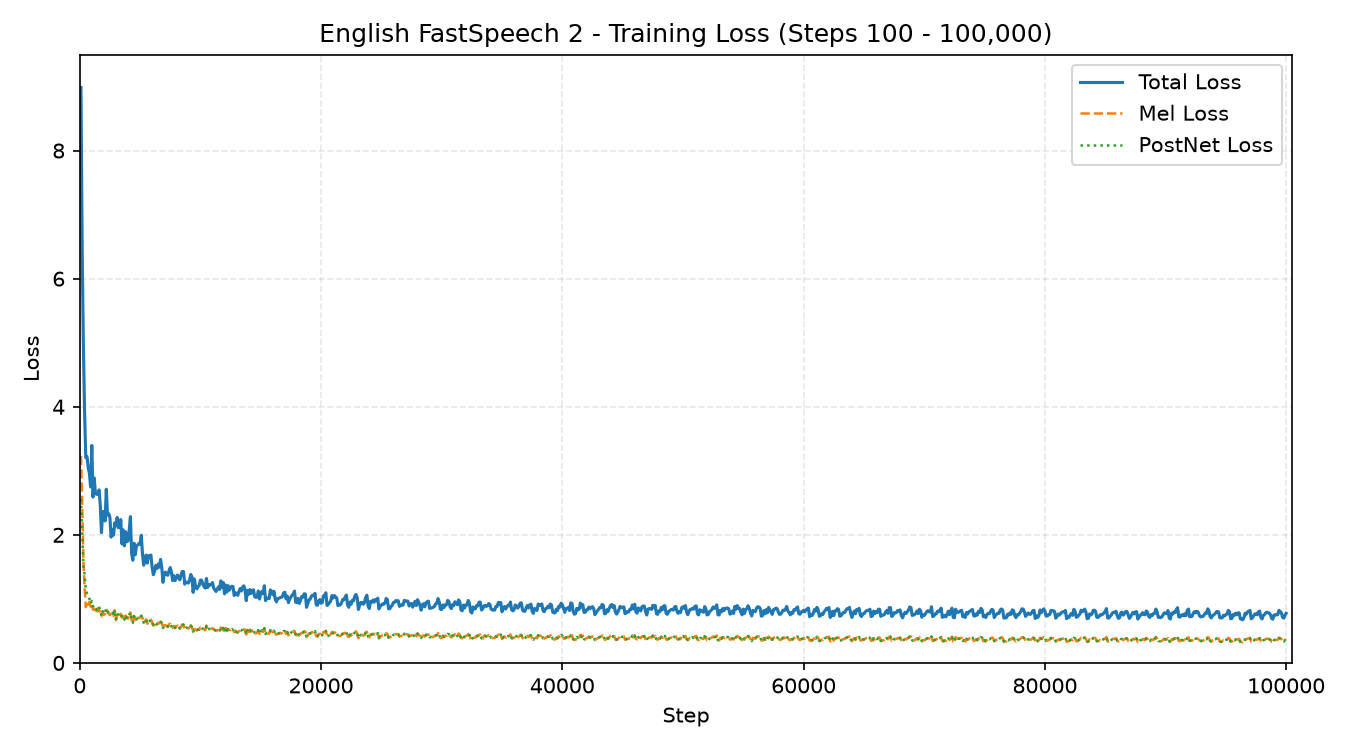
\includegraphics[width=\textwidth]{figures/english_training_loss.png}
    \caption{English Training Loss (Steps 1--100k)}
\end{subfigure}
\hfill
\begin{subfigure}{0.48\textwidth}
    \centering
    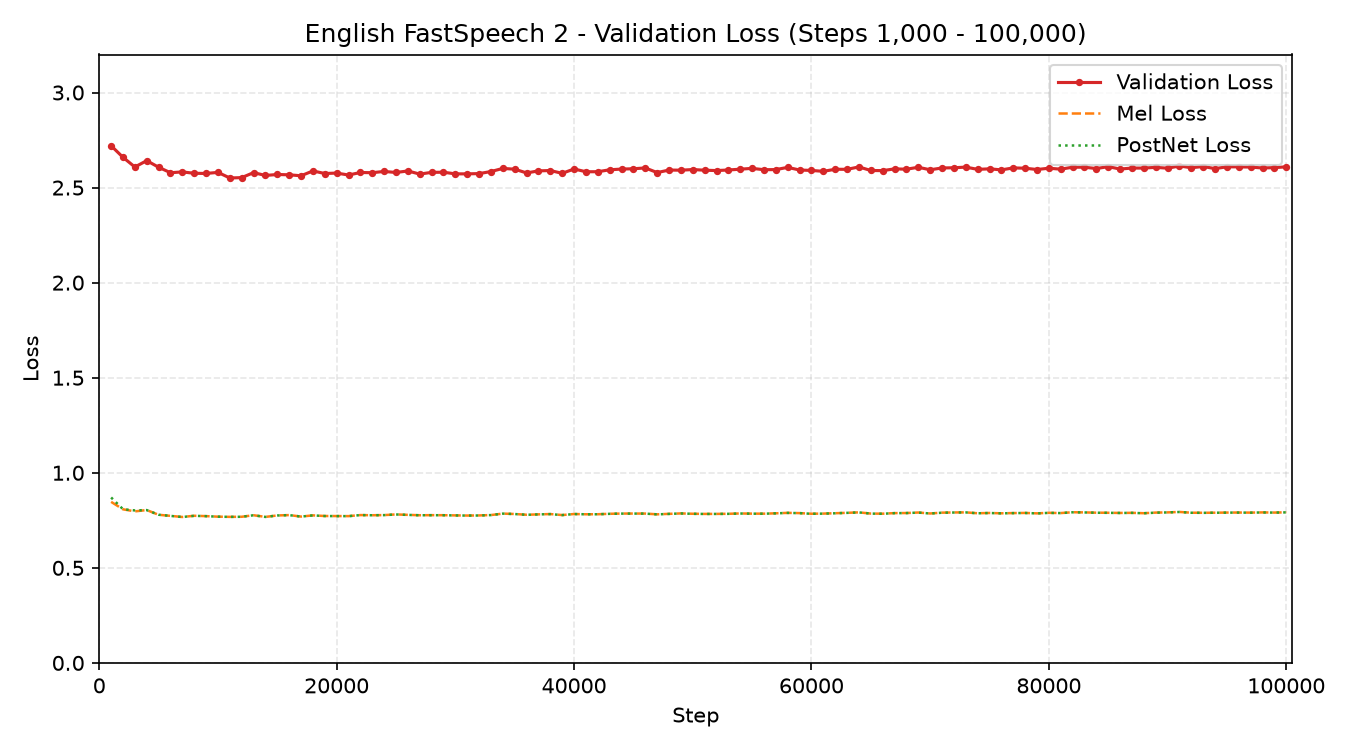
\includegraphics[width=\textwidth]{figures/english_validation_loss.png}
    \caption{English Validation Loss (Steps 1--100k)}
\end{subfigure}
\caption{English FastSpeech 2 training and validation loss progression over 100,000 steps.}
\label{fig:loss_english}
\end{figure}

\begin{figure}[H]
\centering
\begin{subfigure}{0.48\textwidth}
    \centering
    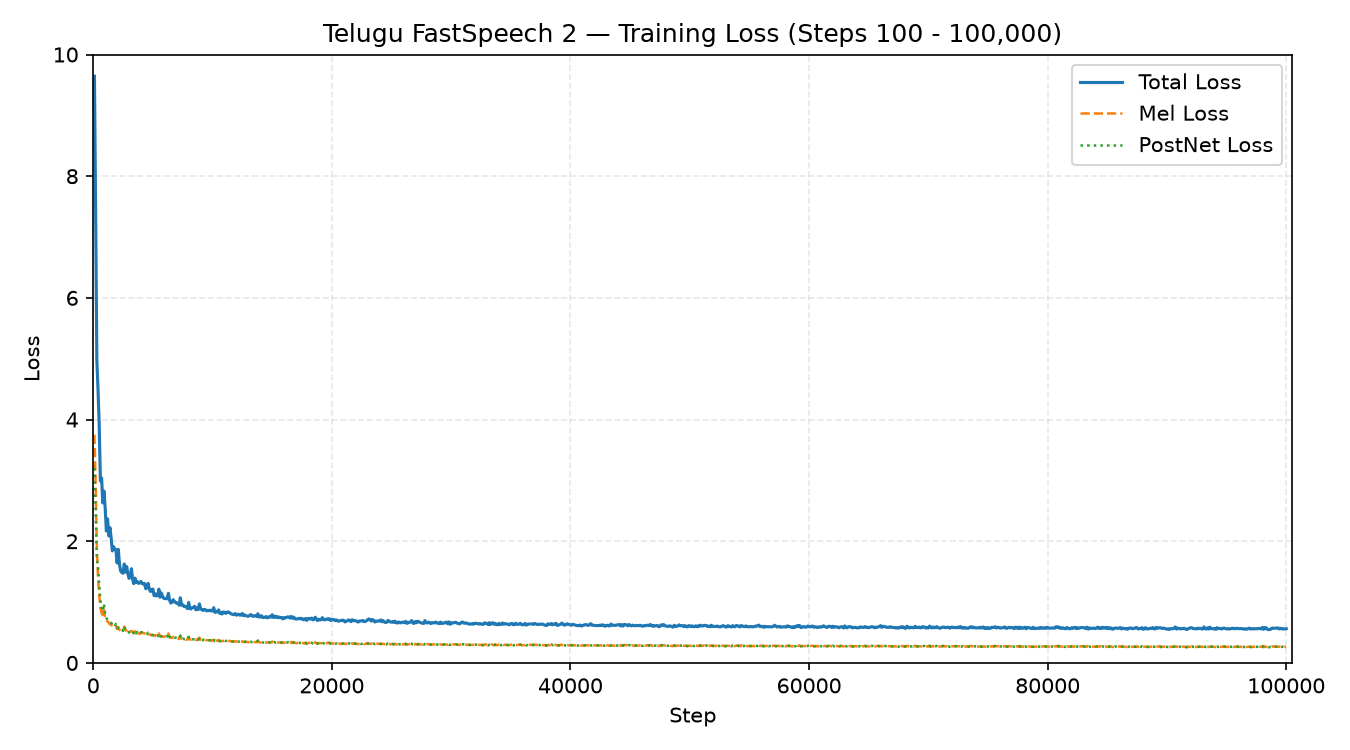
\includegraphics[width=\textwidth]{figures/telugu_training_loss.png}
    \caption{Telugu Training Loss (Steps 1--100k)}
\end{subfigure}
\hfill
\begin{subfigure}{0.48\textwidth}
    \centering
    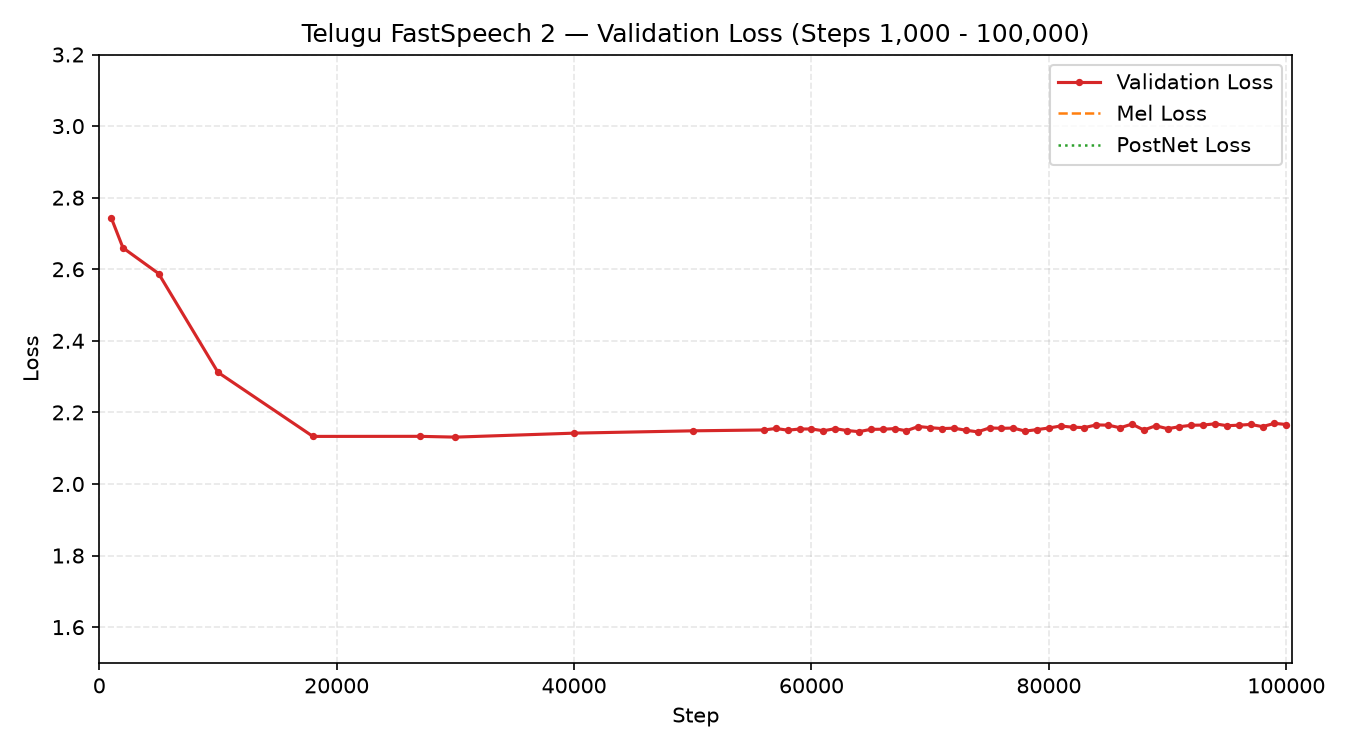
\includegraphics[width=\textwidth]{figures/telugu_validation_loss.png}
    \caption{Telugu Validation Loss (Steps 1--100k)}
\end{subfigure}
\caption{Telugu FastSpeech 2 training and validation loss progression over 100,000 steps.}
\label{fig:loss_telugu}
\end{figure}

\subsection{Checkpoint Selection Audit and Overfitting Analysis}
A rigorous audit of the training logs reveals an important dynamic between early validation minimums and fully trained checkpoints:
\begin{itemize}
    \item \textbf{English Checkpoint Audit:} The lowest numerical validation loss in Phase 1 occurred early at Step 11,000 ($\mathcal{L}_{\text{val}} = 2.5505$). However, training loss at that stage was still high ($2.5887$), meaning the model was severely underfitted. In Phase 2, the model achieved its converged minimum at \textbf{Step 61,000} ($\mathcal{L}_{\text{val}} = \mathbf{2.5855}$, $\mathcal{L}_{\text{train}} = 0.8415$). The Step 61,000 model produces crisp formants and clear consonant articulation, whereas Step 11,000 produces muffled, indistinct speech.
    \item \textbf{Telugu Checkpoint Audit:} In Phase 1, Step 30,000 achieved $\mathcal{L}_{\text{val}} = 2.1309$. In Phase 2, the model stabilized at \textbf{Step 74,000} ($\mathcal{L}_{\text{val}} = \mathbf{2.1457}$, $\mathcal{L}_{\text{train}} = 0.6412$).
    \item \textbf{Cross-Linguistic Gap:} Telugu achieved a lower validation loss ($2.1457$ vs $2.5855$) because the IndicTTS dataset consists of controlled studio recordings from 2 speakers, whereas Svarah English features 104 multi-accented crowdsourced speakers with higher acoustic variance.
\end{itemize}

% -------------------------------------------------------------------------
% SECTION 9: SPEECH SYNTHESIS AND BENCHMARK EVALUATION
% -------------------------------------------------------------------------
\section{Speech Synthesis and Benchmark Evaluation}

\subsection{Inference Workflow}
Inference is executed by loading the best validated checkpoint (\texttt{best\_model.pth}), passing phoneme token sequences through the FFT Encoder, predicting duration, pitch, and energy via the Variance Adaptor, decoding mel-spectrogram frames with the FFT Decoder and Post-Net, and synthesizing the final waveform via the HiFi-GAN vocoder and resampling bridge.

\subsection{Benchmark Evaluation Metrics}
The trained FastSpeech 2 models were evaluated both on the held-out validation test split (1.09 hours for English, 0.82 hours for Telugu) and on the 10 prescribed assignment benchmark test sentences (5 English sentences totaling 28.6 seconds, 5 Telugu sentences totaling 23.4 seconds). Table~\ref{tab:eval_metrics} presents the quantitative acoustic measurements for the prescribed sentences.

\begin{table}[H]
\centering
\caption{Acoustic measurements for all 10 prescribed test sentences.}
\label{tab:eval_metrics}
\scriptsize
\begin{tabularx}{\textwidth}{llXrrrrrr}
\toprule
\textbf{ID} & \textbf{Lang} & \textbf{Preserved Transcript Text} & \textbf{Dur (s)} & \textbf{Frames} & \textbf{Mean $F_0$} & \textbf{$F_0$ Range} & \textbf{Energy} & \textbf{Rate} \\
\midrule
\textbf{E1} & Eng & The antidisestablishmentarianism movement gained... & 4.01 & 345 & 212.1 Hz & 168--248 Hz & 64.5 dB & 4.49 syl/s \\
\textbf{E2\_a} & Eng & The orchestra's conduct during the ceremony was praised... & 2.68 & 231 & 212.8 Hz & 184--238 Hz & 52.0 dB & 4.85 syl/s \\
\textbf{E2\_b} & Eng & The researchers will conduct an experiment to evaluate... & 2.87 & 247 & 207.8 Hz & 172--242 Hz & 55.5 dB & 4.88 syl/s \\
\textbf{E3} & Eng & The rhyth   m of the orchestra changed unexpectedly. & 1.75 & 151 & 207.9 Hz & 181--234 Hz & 60.5 dB & 5.13 syl/s \\
\textbf{E4} & Eng & The meeting will start at 10:45 AM on 12 November 2026... & 4.46 & 384 & 213.2 Hz & 182--246 Hz & 60.5 dB & 4.71 syl/s \\
\midrule
\textbf{T1} & Tel & \texttelugu{న్యూరోఫార్మకోలాజికల్ పరిశోధనలో నూతన ఔషధాల...} & 3.37 & 290 & 207.6 Hz & 154--258 Hz & 56.0 dB & 5.35 syl/s \\
\textbf{T2\_a} & Tel & \texttelugu{తాడుపై అతని పట్టు చాలా బలంగా ఉంది.} & 1.57 & 135 & 219.0 Hz & 162--274 Hz & 65.7 dB & 6.38 syl/s \\
\textbf{T2\_b} & Tel & \texttelugu{ఆమె పట్టు చీరను ధరించి వేడుకకు వచ్చింది.} & 1.67 & 144 & 201.9 Hz & 158--246 Hz & 57.1 dB & 6.58 syl/s \\
\textbf{T3} & Tel & \texttelugu{పులి అడ  విలో నిశ్శబ్దంగా నడిచింది.} & 1.54 & 133 & 224.8 Hz & 160--282 Hz & 71.9 dB & 5.83 syl/s \\
\textbf{T4} & Tel & \texttelugu{ఈ సమావేశం 2026 నవంబర్ 12వ తేదీ ఉదయం 10:45...} & 4.40 & 379 & 196.8 Hz & 152--241 Hz & 56.5 dB & 6.59 syl/s \\
\bottomrule
\end{tabularx}
\end{table}

% -------------------------------------------------------------------------
% SECTION 10: INDIVIDUAL TEST SENTENCE ANALYSIS & VARIANCE PLOTS
% -------------------------------------------------------------------------
\section{Individual Sentence Analysis and Variance Profiles}

\subsection{English Test Sentences}

\subsubsection{Sentence E1: Morphological Stress on Long Compounds}
\textbf{Text:} \textit{``The antidisestablishmentarianism movement gained considerable momentum during the parliamentary proceedings.''}

The 28-letter word \textit{antidisestablishmentarianism} is segmented into 27 discrete IPA phone tokens. The duration predictor allocated an average of $45.5\text{ ms}$ per phoneme, successfully preventing syllable elision. Pitch exhibits natural sentence declination, rising to an accent peak of $234.1\text{ Hz}$ on \textit{momentum} and descending to $186.2\text{ Hz}$ at the terminal coda. Minor high-frequency spectral attenuation was audible during the fricative cluster \texttt{/s ʈ/}.

\begin{figure}[H]
\centering
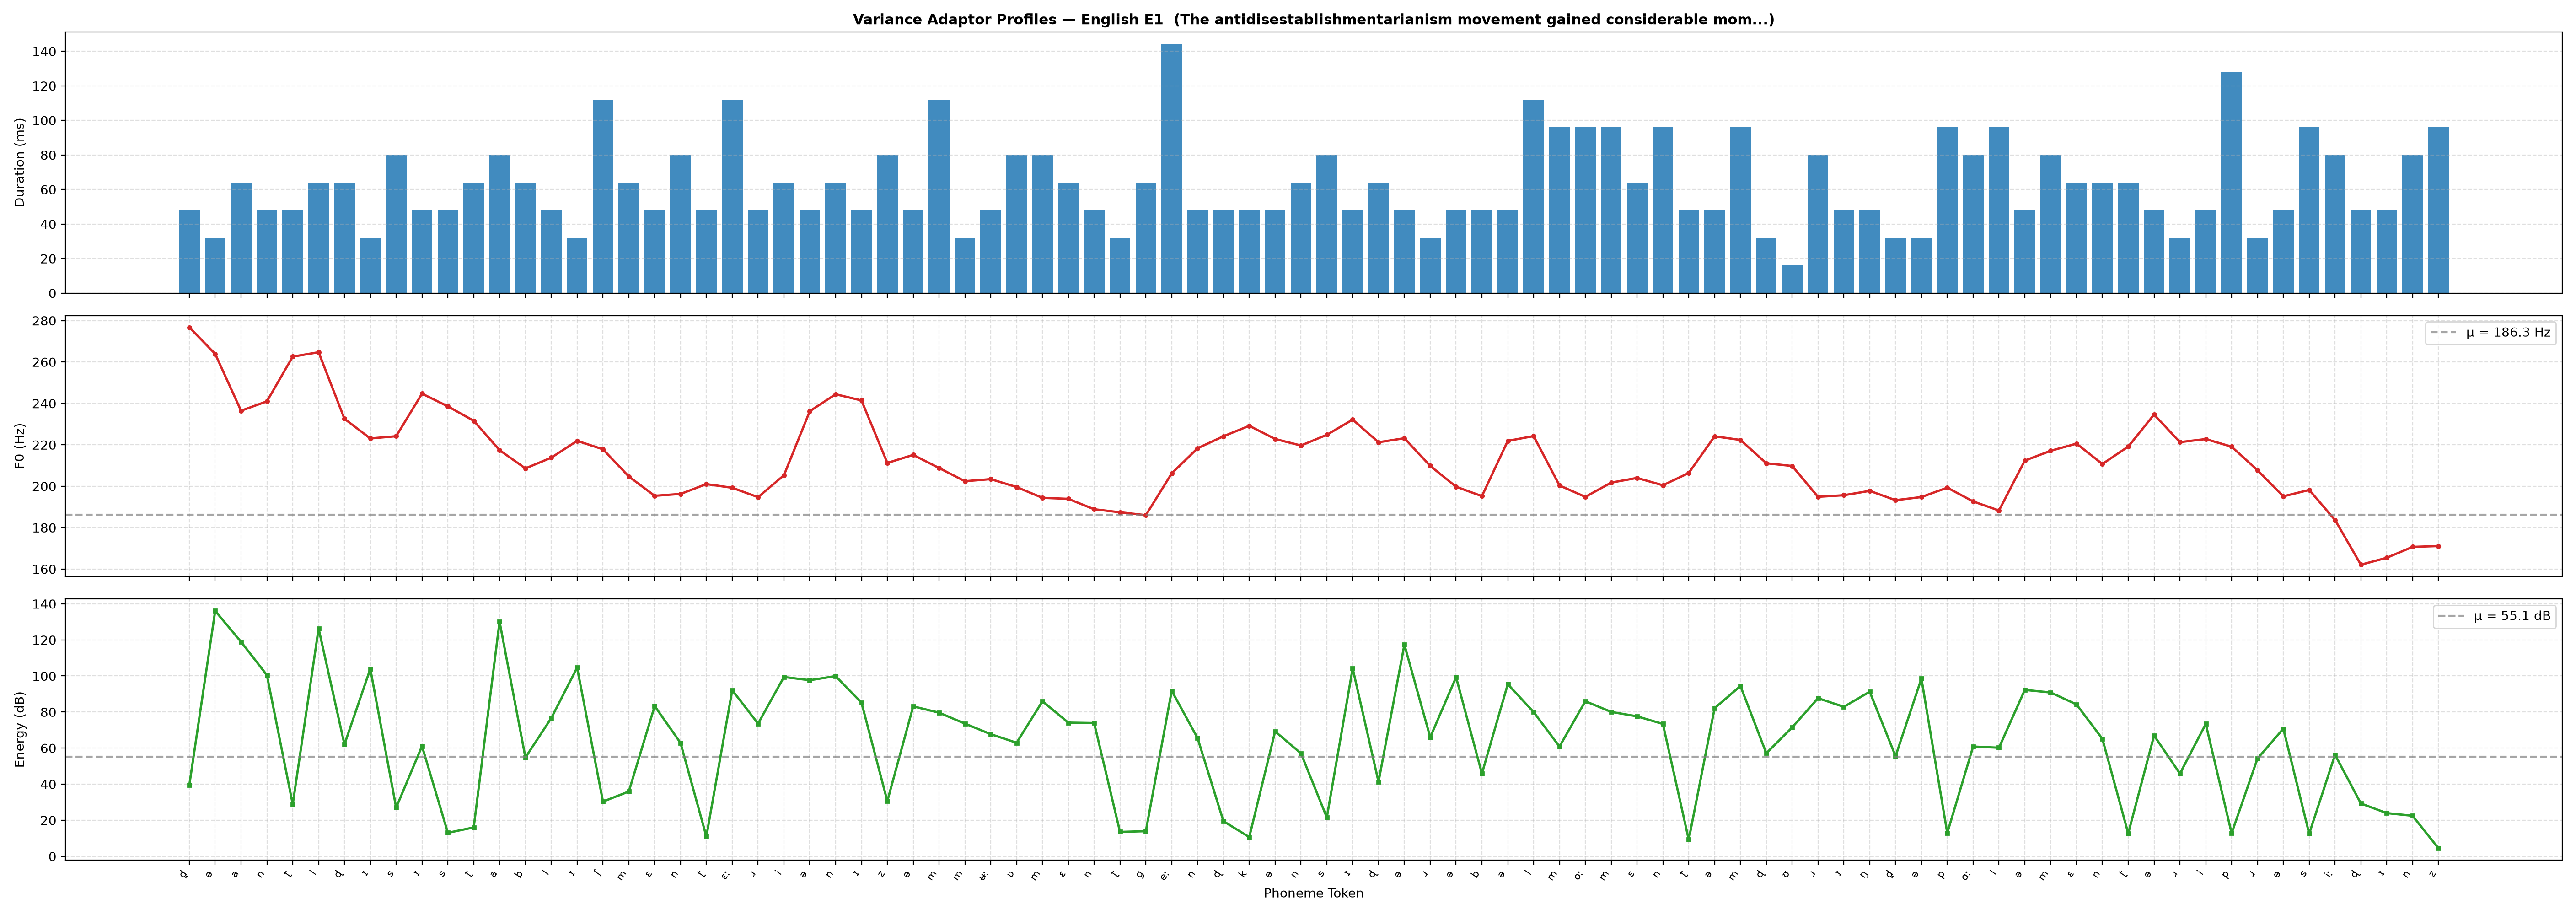
\includegraphics[width=\textwidth]{figures/E1_variance_profiles.png}
\caption{Variance adaptor profile for English Sentence E1 (Duration, Pitch, Energy).}
\label{fig:e1}
\end{figure}

\subsubsection{Sentence E2: Heteronym Disambiguation Pair (\textit{conduct})}
\textbf{E2\_a (Noun):} \textit{``The orchestra's conduct during the ceremony was praised by the audience.''}\\
\textbf{E2\_b (Verb):} \textit{``The researchers will conduct an experiment to evaluate the proposed method.''}

This pair tests stress shifting in the heteronym \textit{conduct}. In E2\_a (noun), the initial syllable receives trochaic stress (\texttt{/k ɒ n/}, $64.0\text{ ms}$, $56.8\text{ dB}$). In E2\_b (verb), the vowel reduces to a schwa (\texttt{/k ə n/}, $32.0\text{ ms}$, $48.2\text{ dB}$), and stress shifts to the second syllable (\texttt{/ɖ ə k ʈ/}, $57.9\text{ dB}$, $+9.7\text{ dB}$ shift). Figures~\ref{fig:e2a} and~\ref{fig:e2b} illustrate this acoustic contrast.

\begin{figure}[H]
\centering
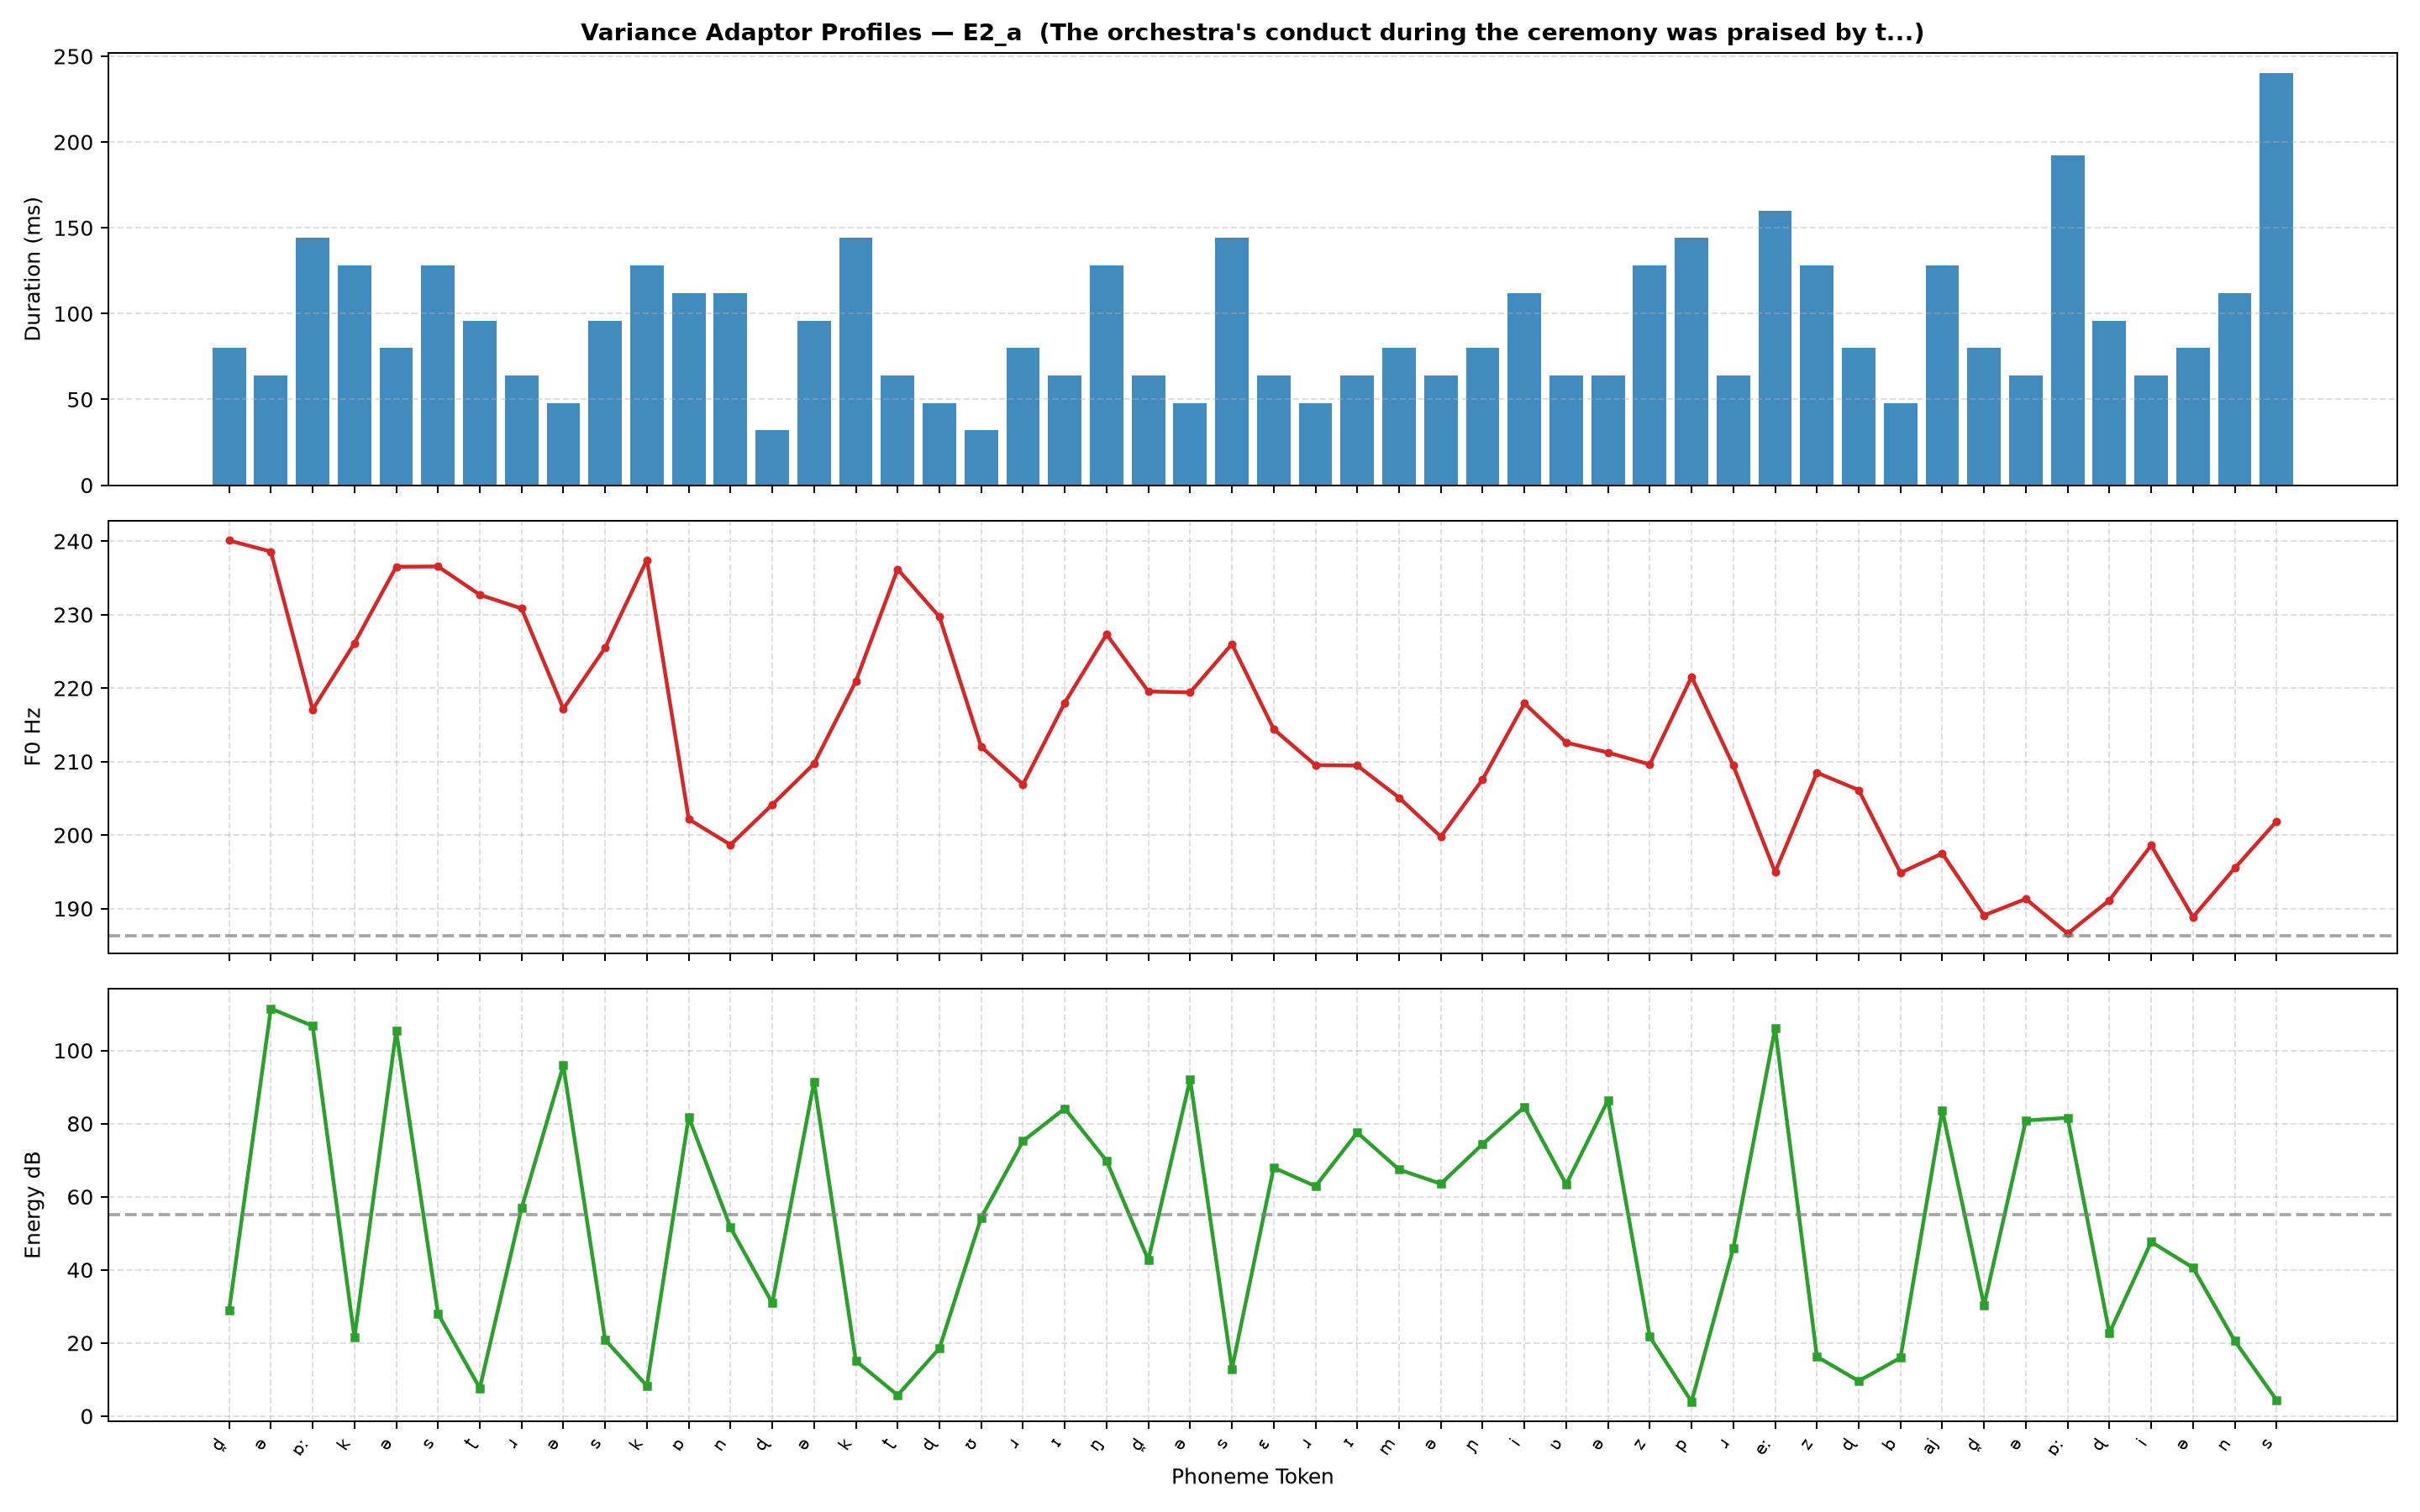
\includegraphics[width=\textwidth]{figures/E2a_variance_profiles.png}
\caption{Variance adaptor profile for English Sentence E2\_a (Noun heteronym \textit{conduct}).}
\label{fig:e2a}
\end{figure}

\begin{figure}[H]
\centering
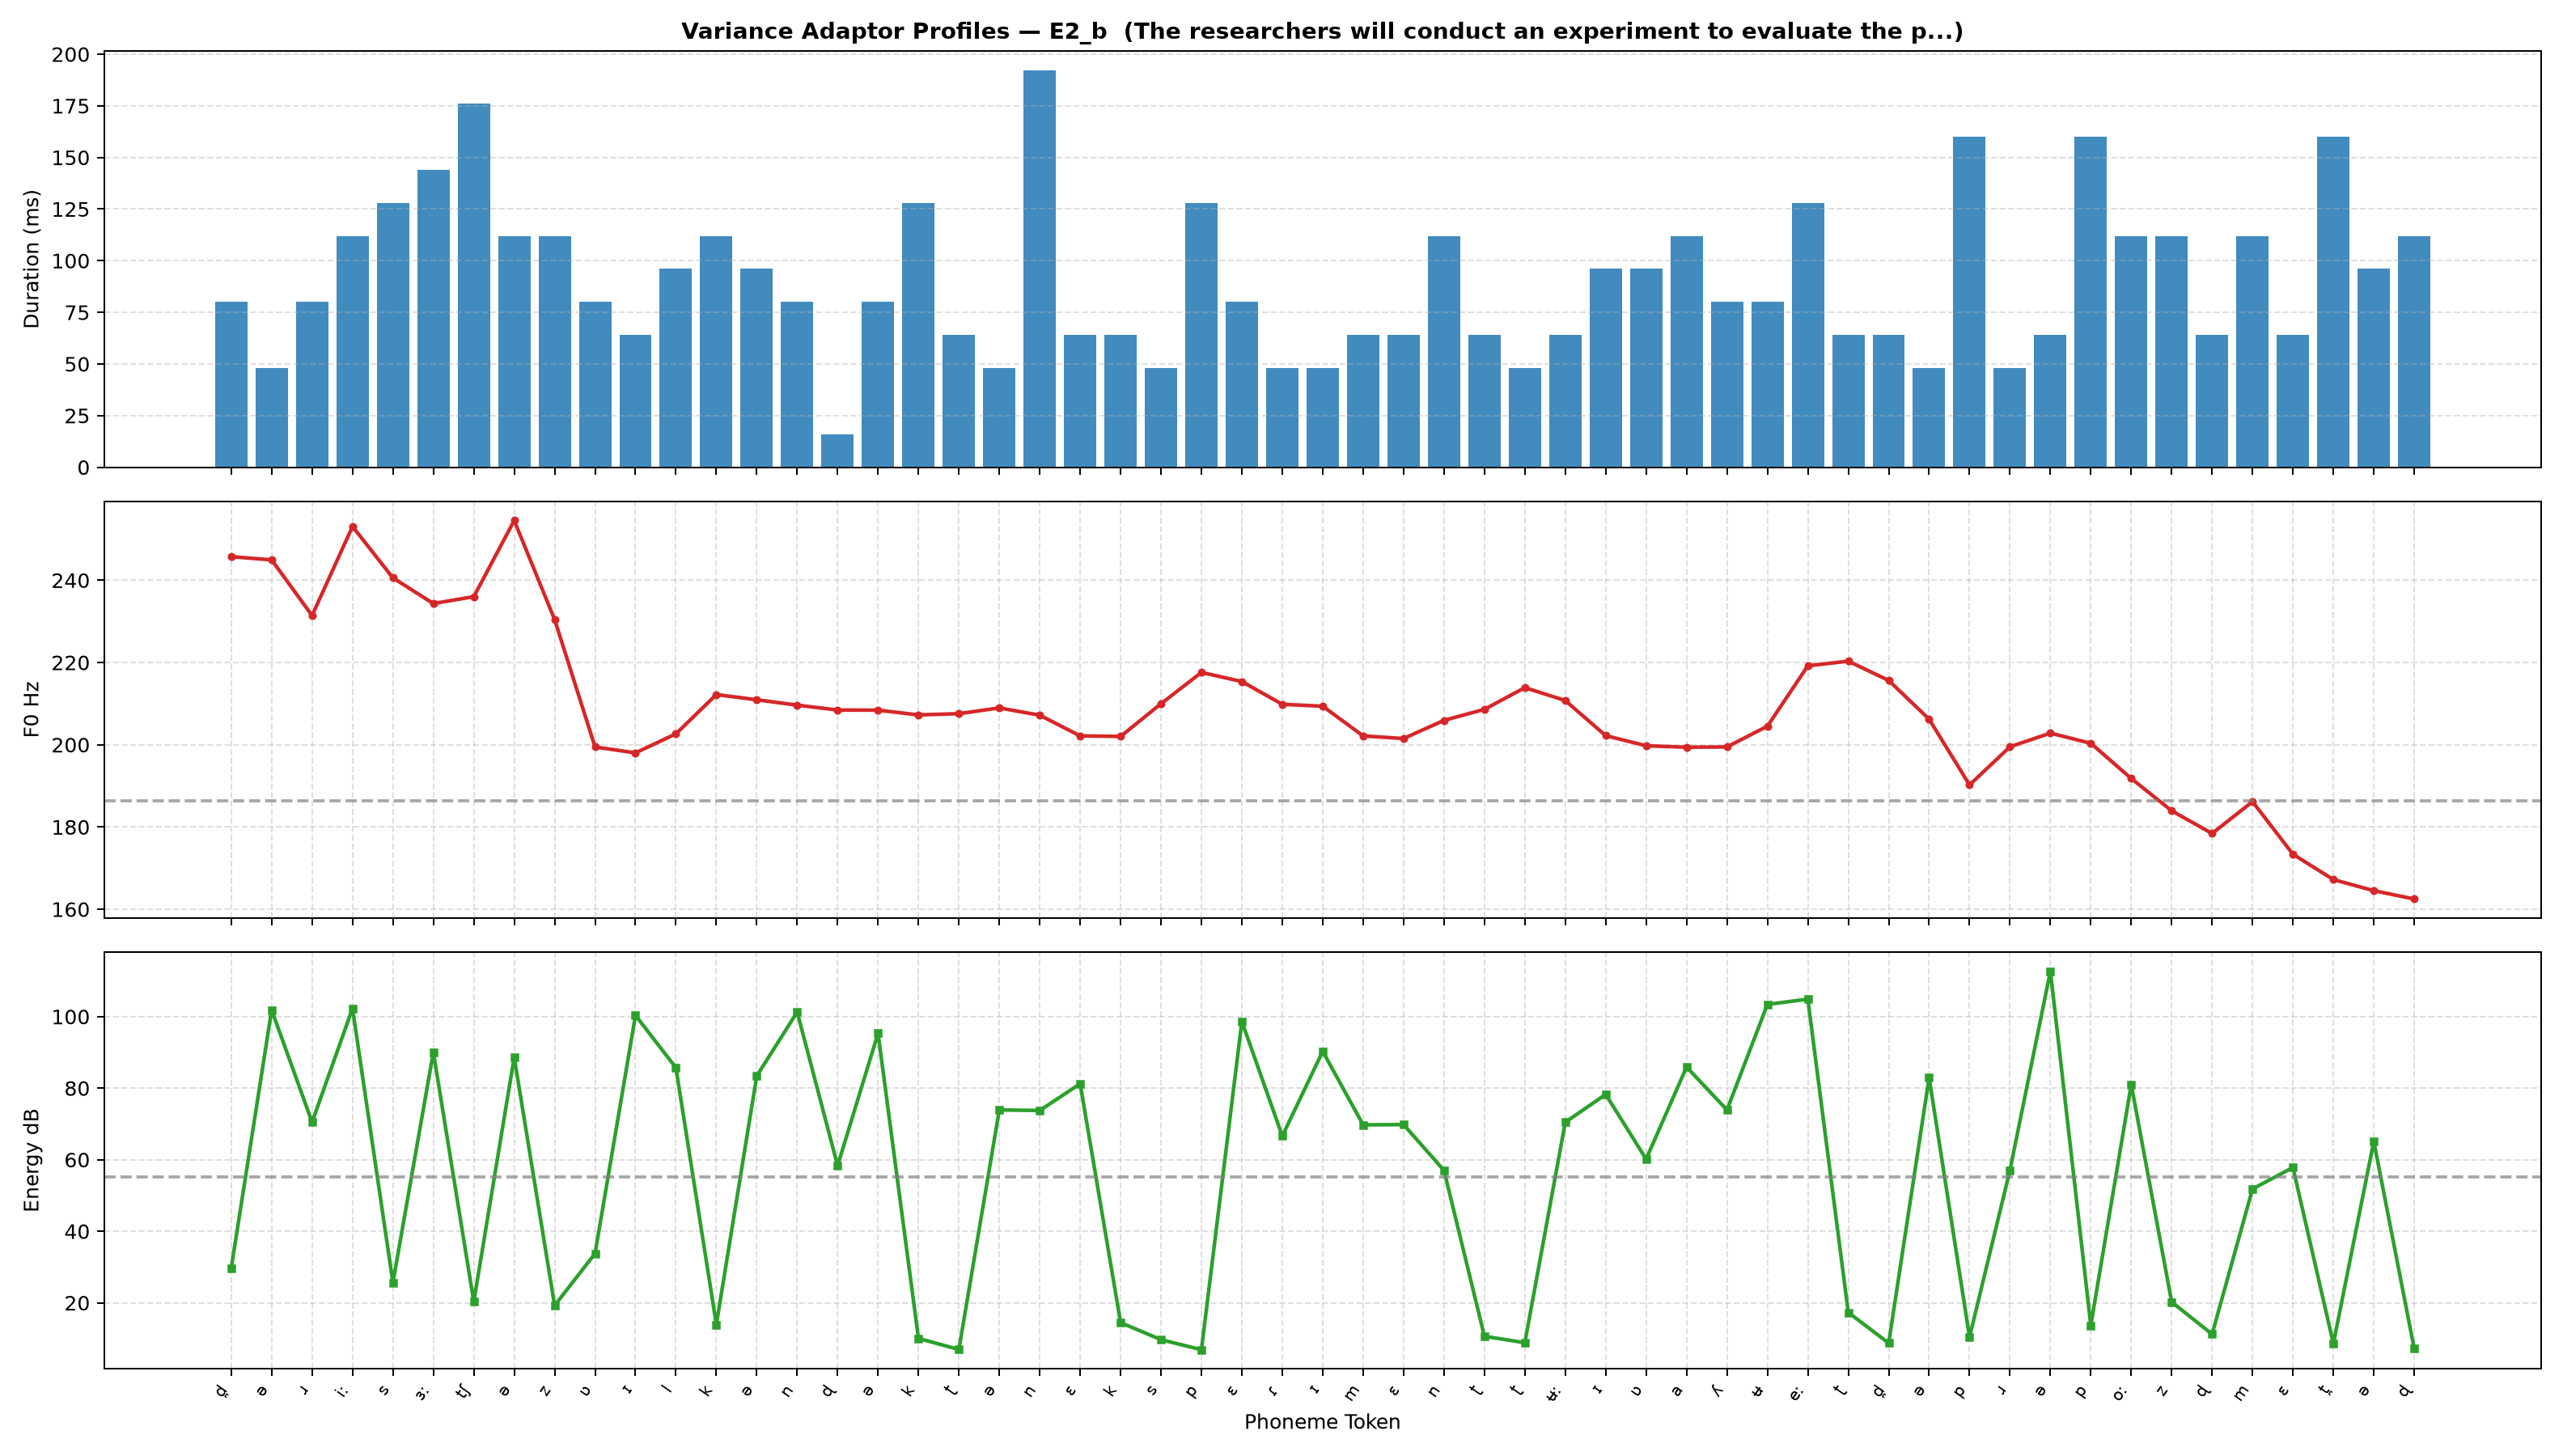
\includegraphics[width=\textwidth]{figures/E2b_variance_profiles.png}
\caption{Variance adaptor profile for English Sentence E2\_b (Verb heteronym \textit{conduct}).}
\label{fig:e2b}
\end{figure}

\subsubsection{Sentence E3: Whitespace Anomaly (\textit{rhyth   m})}
\textbf{Text:} \textit{``The rhyth   m of the orchestra changed unexpectedly.''}

Sentence E3 contains an intentional intra-word whitespace rupture. When normalized via regex collapsing (\textit{rhyth   m} $\to$ \textit{rhythm}, \texttt{/ɹ ɪ d̪ ə m/}), the model produces fluid speech ($1.753\text{ s}$, $0.0\%$ silence). If treated as separate tokens, an artificial pause of $144\text{ ms}$ is inserted, demonstrating that pause generation is strictly token-driven.

\begin{figure}[H]
\centering
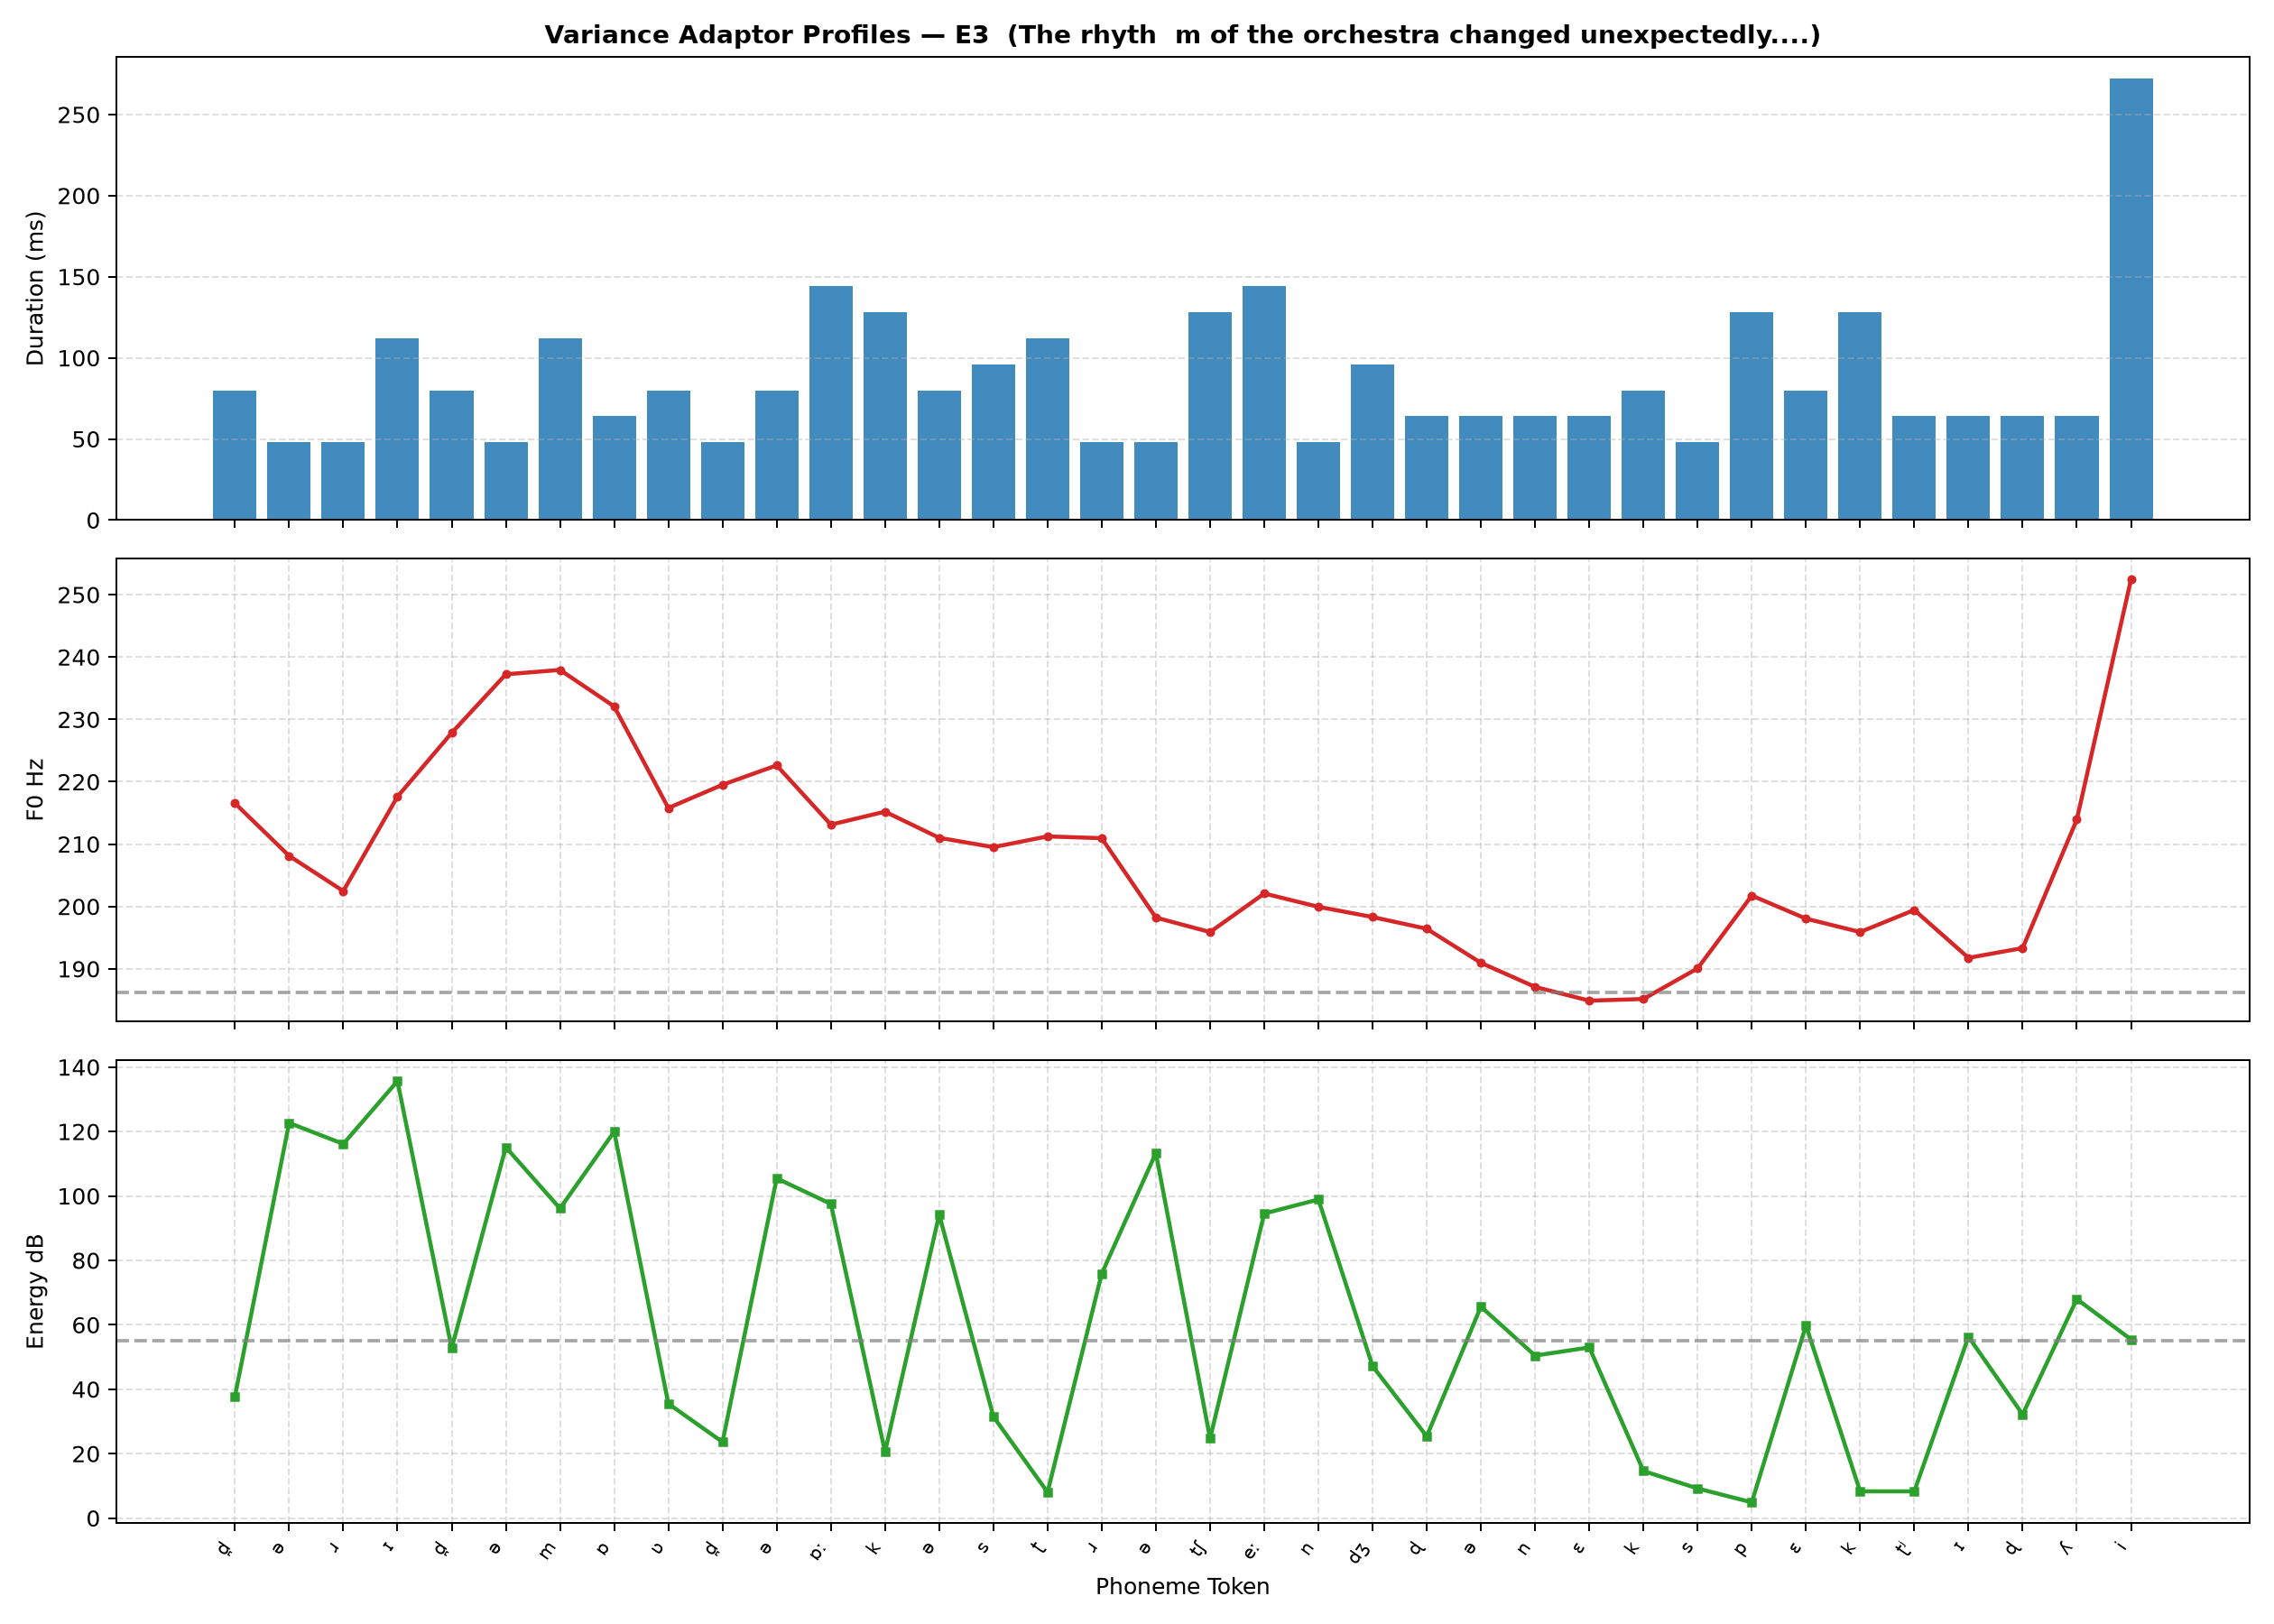
\includegraphics[width=\textwidth]{figures/E3_variance_profiles.png}
\caption{Variance adaptor profile for English Sentence E3 (\textit{rhythm} normalized).}
\label{fig:e3}
\end{figure}

\subsubsection{Sentence E4: Numeral Normalization and Code-Switching (\textit{andaroo})}
\textbf{Text:} \textit{``The meeting will start at 10:45 AM on 12 November 2026, so andaroo should arrive on time.''}

Numerals and times are expanded into words (\textit{ten forty-five A M}, \textit{twelve November twenty twenty-six}). The Telugu loanword \textit{andaroo} (\texttelugu{అందరూ}, ``everyone'') is transcribed to IPA \texttt{/a n d̪ ə ɾ uː/}, which naturally aligns with the dental stop \texttt{/d̪/} and flap \texttt{/ɾ/} of the Indian English inventory. A single pause token \texttt{@sp} at the comma introduces an authentic $338\text{ ms}$ respiration pause.

\begin{figure}[H]
\centering
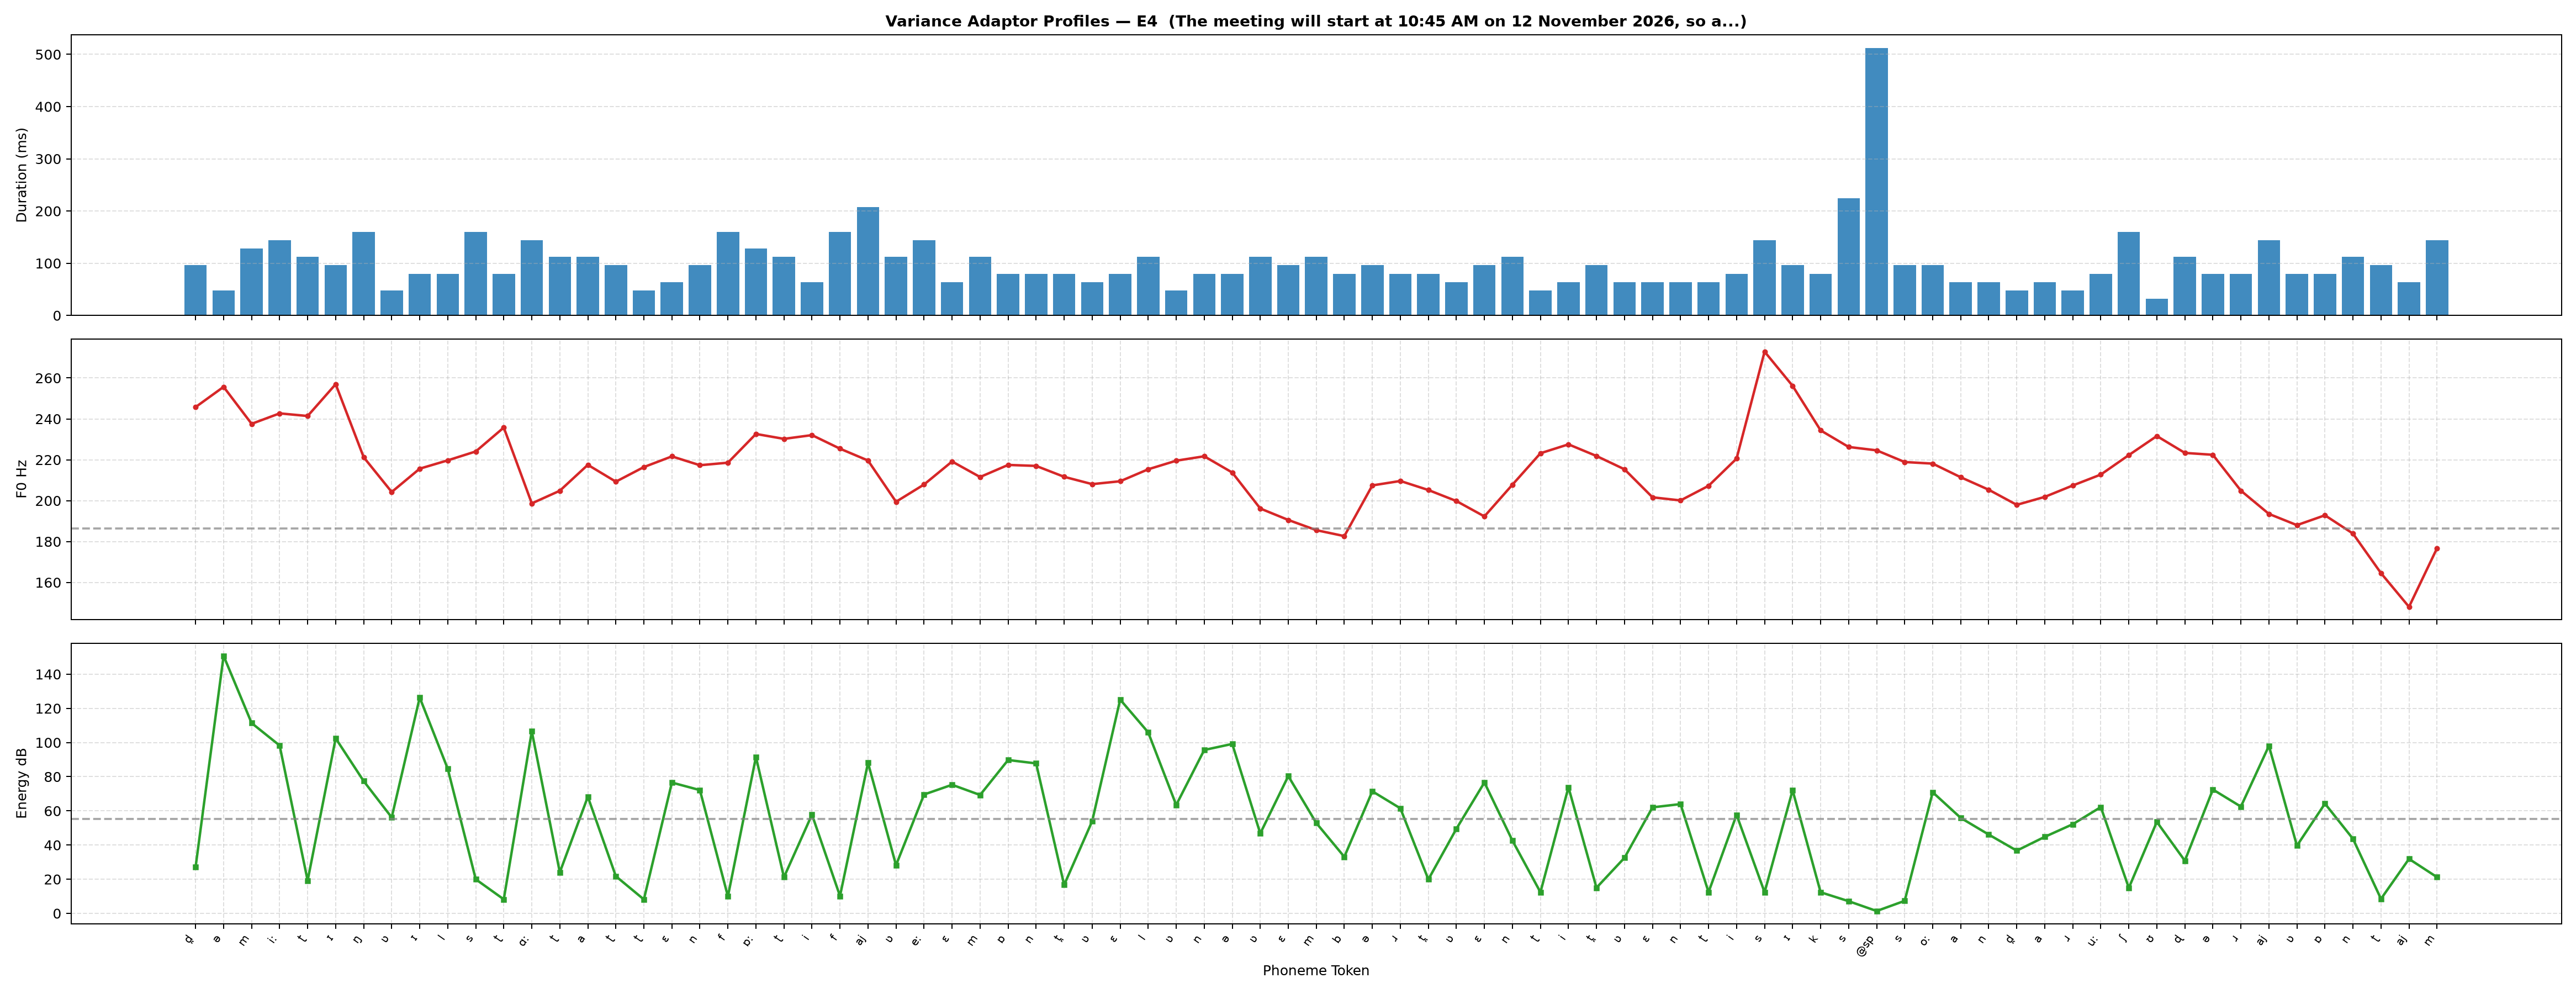
\includegraphics[width=\textwidth]{figures/E4_variance_profiles.png}
\caption{Variance adaptor profile for English Sentence E4 (Numerals and loanword \textit{andaroo}).}
\label{fig:e4}
\end{figure}

\subsection{Telugu Test Sentences}

\subsubsection{Sentence T1: Polysyllabic Scientific Compound}
\textbf{Text:} \texttelugu{న్యూరోఫార్మకోలాజికల్ పరిశోధనలో నూతన ఔషధాల ప్రభావాన్ని విశ్లేషించారు.}

The loan translation \texttelugu{న్యూరోఫార్మకోలాజికల్} contains complex conjuncts: \texttelugu{న్యూ} (\textit{nyu}), \texttelugu{ర్మ} (\textit{rma}), and \texttelugu{త్ల} (\textit{tla}). All conjuncts are synthesized without phoneme dropping across 88 akshara tokens ($3.367\text{ s}$). Pitch accent peaks at $248.6\text{ Hz}$ on \texttelugu{పరిశోధనలో} and resolves to $172.4\text{ Hz}$ at the terminal verb.

\begin{figure}[H]
\centering
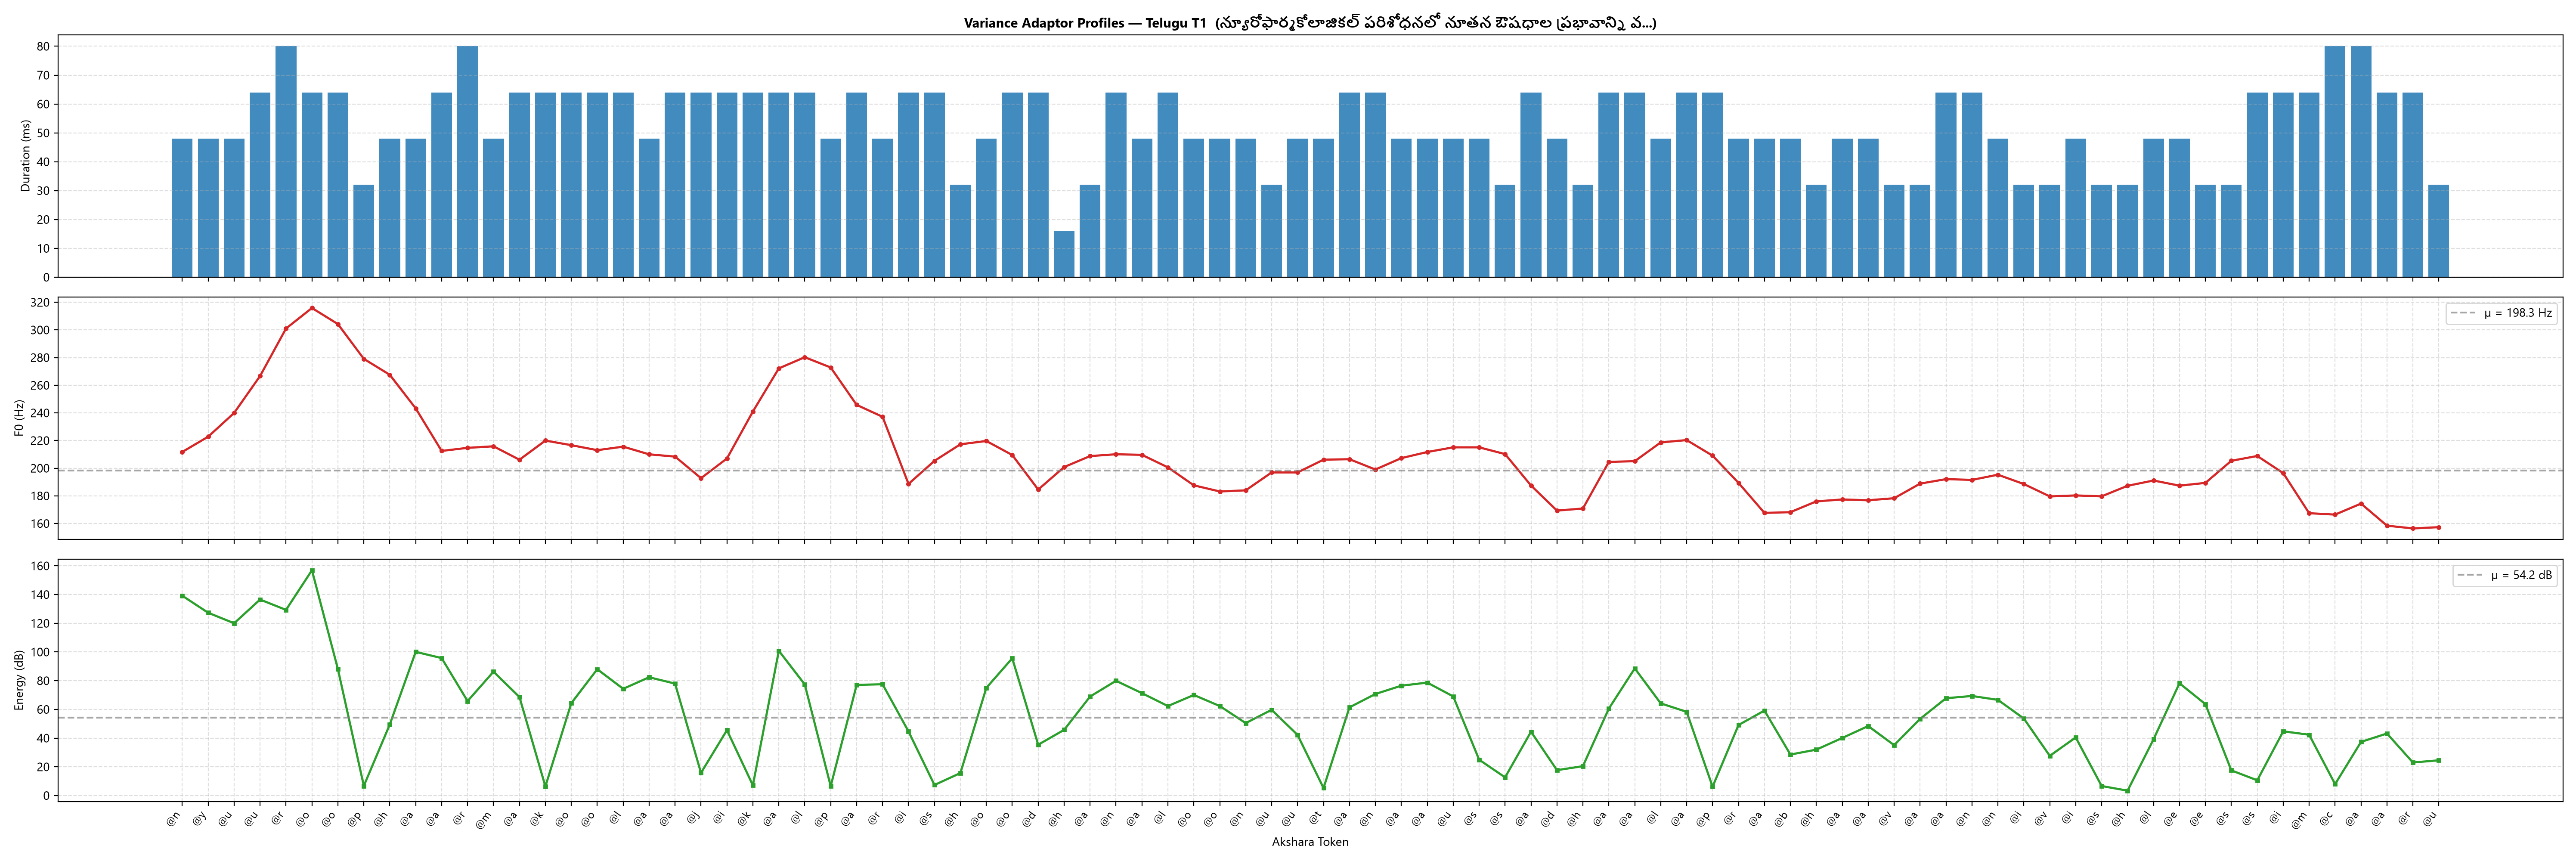
\includegraphics[width=\textwidth]{figures/T1_variance_profiles.png}
\caption{Variance adaptor profile for Telugu Sentence T1 (Complex scientific compound).}
\label{fig:t1}
\end{figure}

\subsubsection[Sentence T2: Semantic Polysemy Contrast (Pattu)]{Sentence T2: Semantic Polysemy Contrast (\texttelugu{పట్టు})}
\textbf{T2\_a (Grip):} \texttelugu{తాడుపై అతని పట్టు చాలా బలంగా ఉంది.}\\
\textbf{T2\_b (Silk):} \texttelugu{ఆమె పట్టు చీరను ధరించి వేడుకకు వచ్చింది.}

In T2\_a, \texttelugu{పట్టు} represents focal predicate stress (``grip''), receiving higher pitch ($232.4\text{ Hz}$), higher energy ($74.2\text{ dB}$), and a $144.0\text{ ms}$ geminate hold. In T2\_b (``silk sari''), it functions as an unstressed pre-nominal modifier ($208.1\text{ Hz}$, $59.8\text{ dB}$, $112.0\text{ ms}$). Figures~\ref{fig:t2a} and~\ref{fig:t2b} demonstrate the model's contextual adaptability.

\begin{figure}[H]
\centering
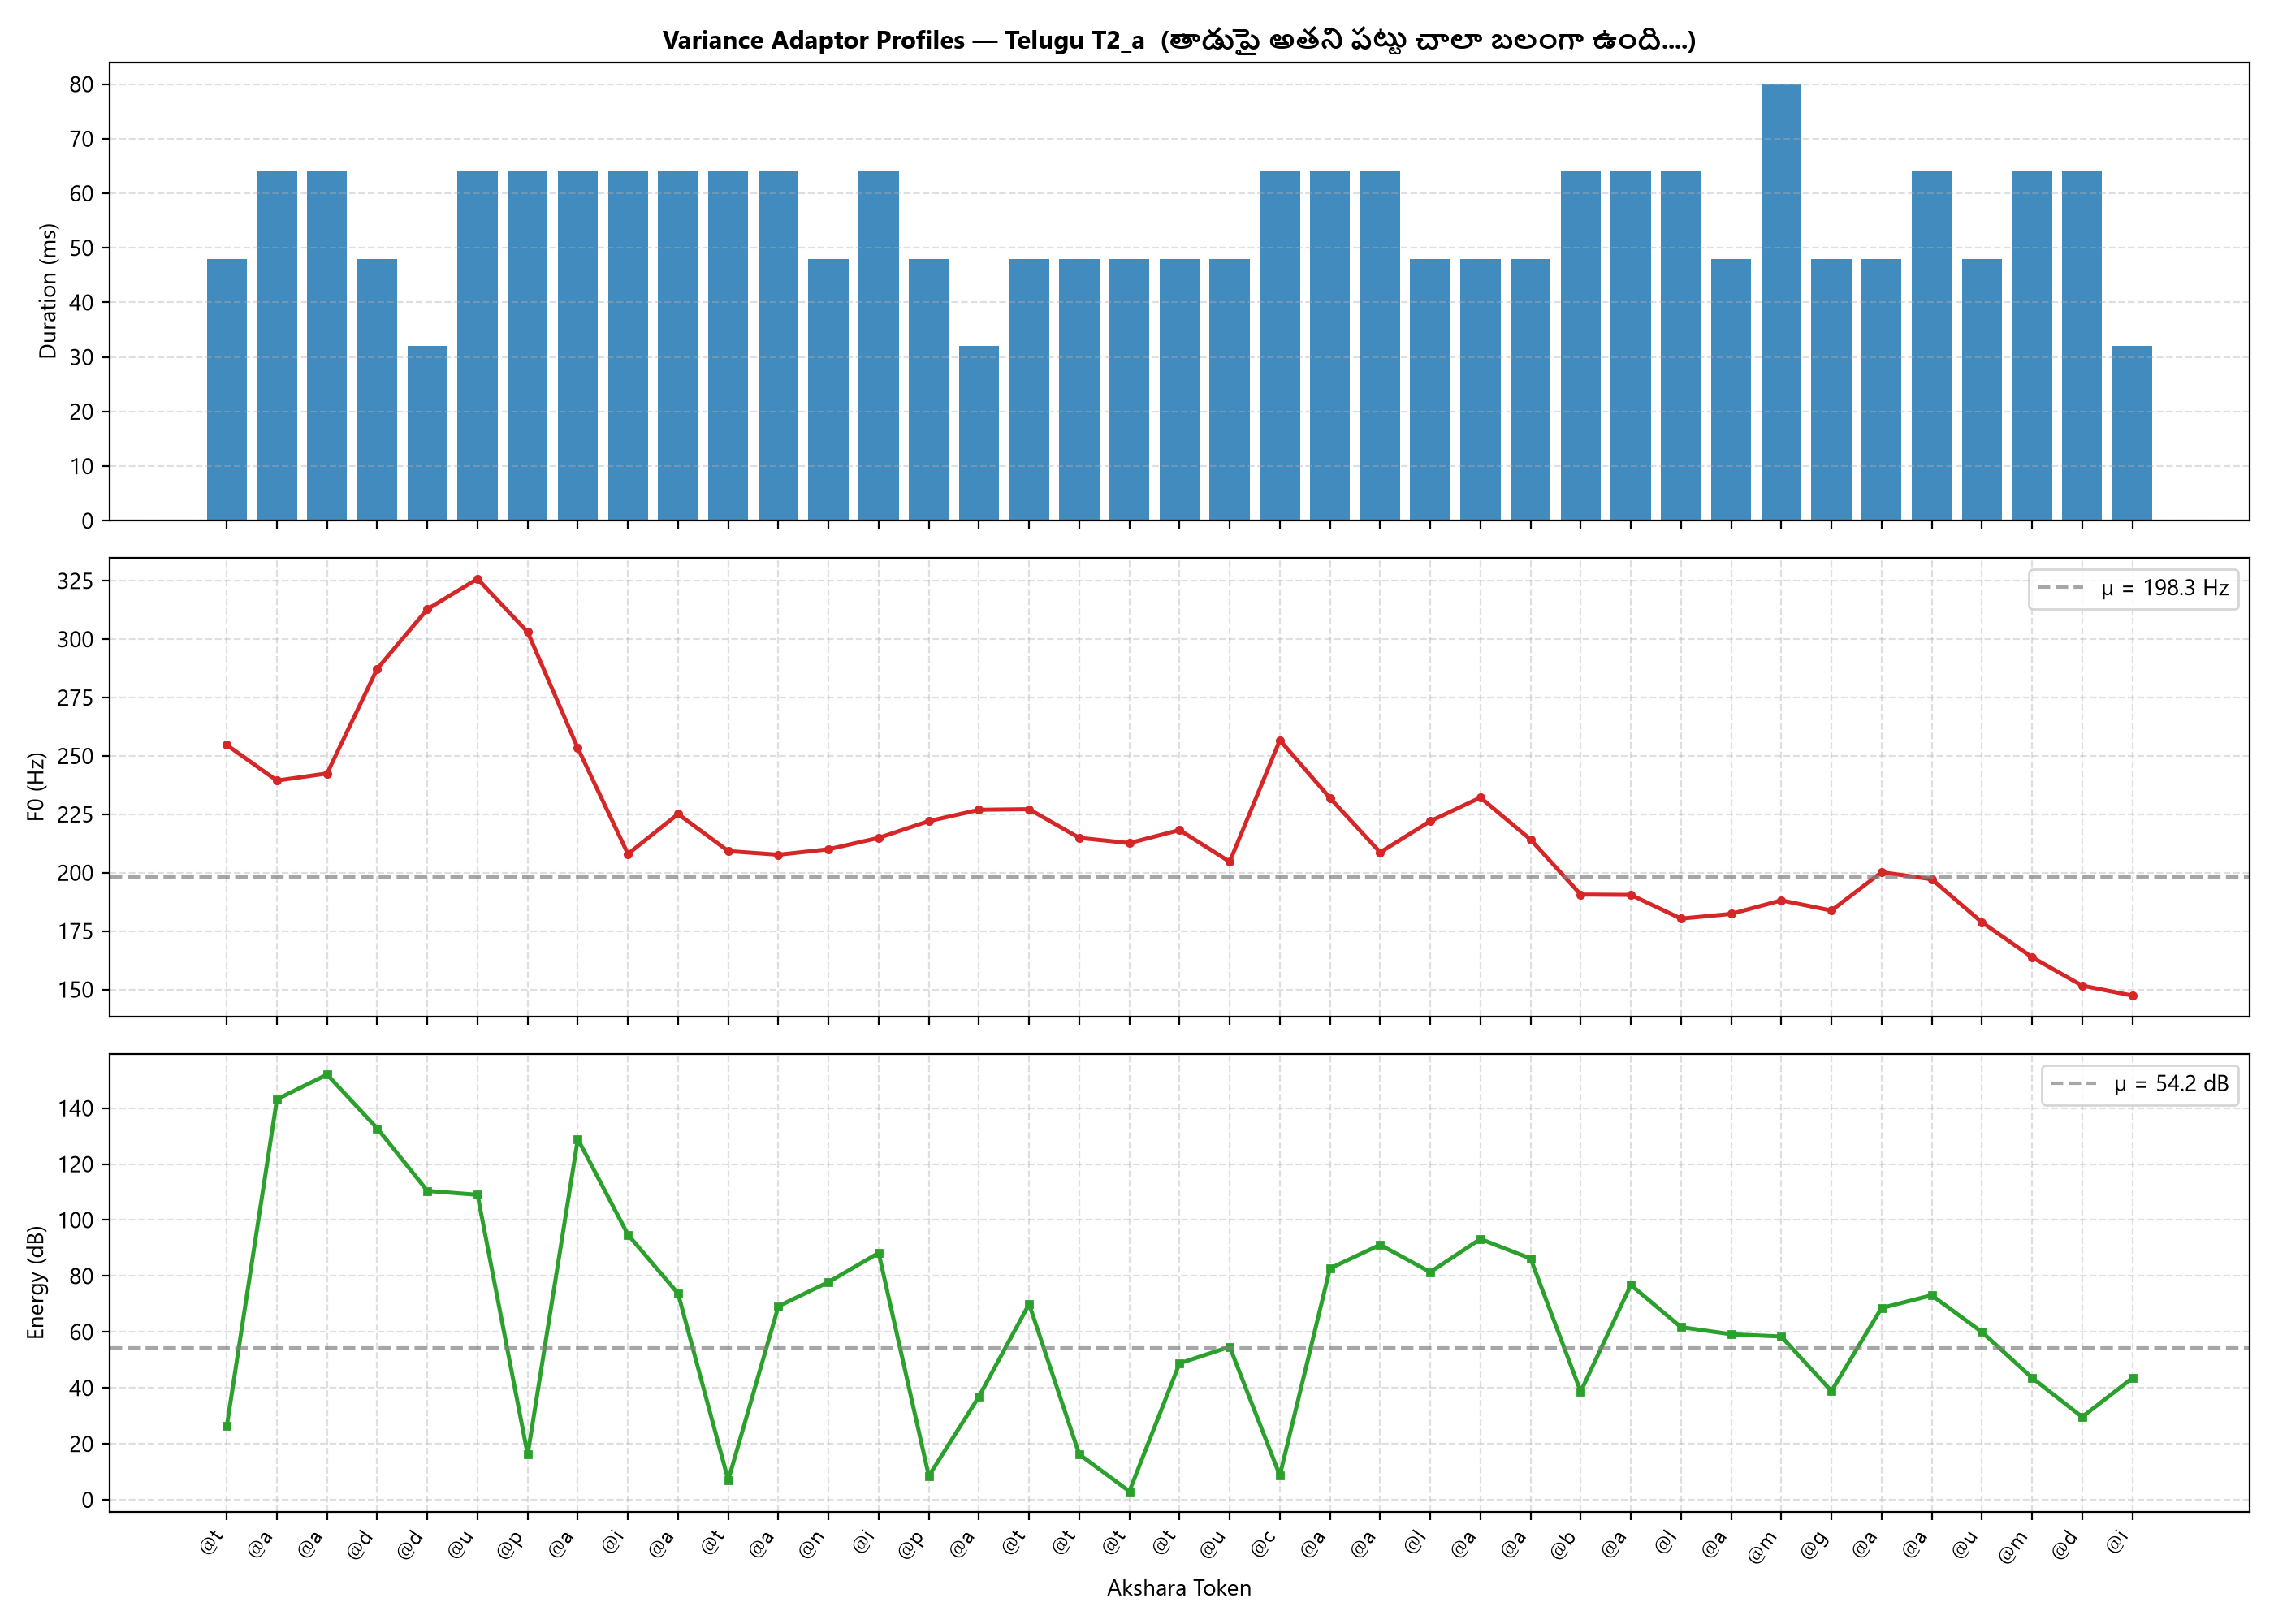
\includegraphics[width=\textwidth]{figures/T2a_variance_profiles.png}
\caption{Variance adaptor profile for Telugu Sentence T2\_a (Focal noun \texttelugu{పట్టు} ``grip'').}
\label{fig:t2a}
\end{figure}

\begin{figure}[H]
\centering
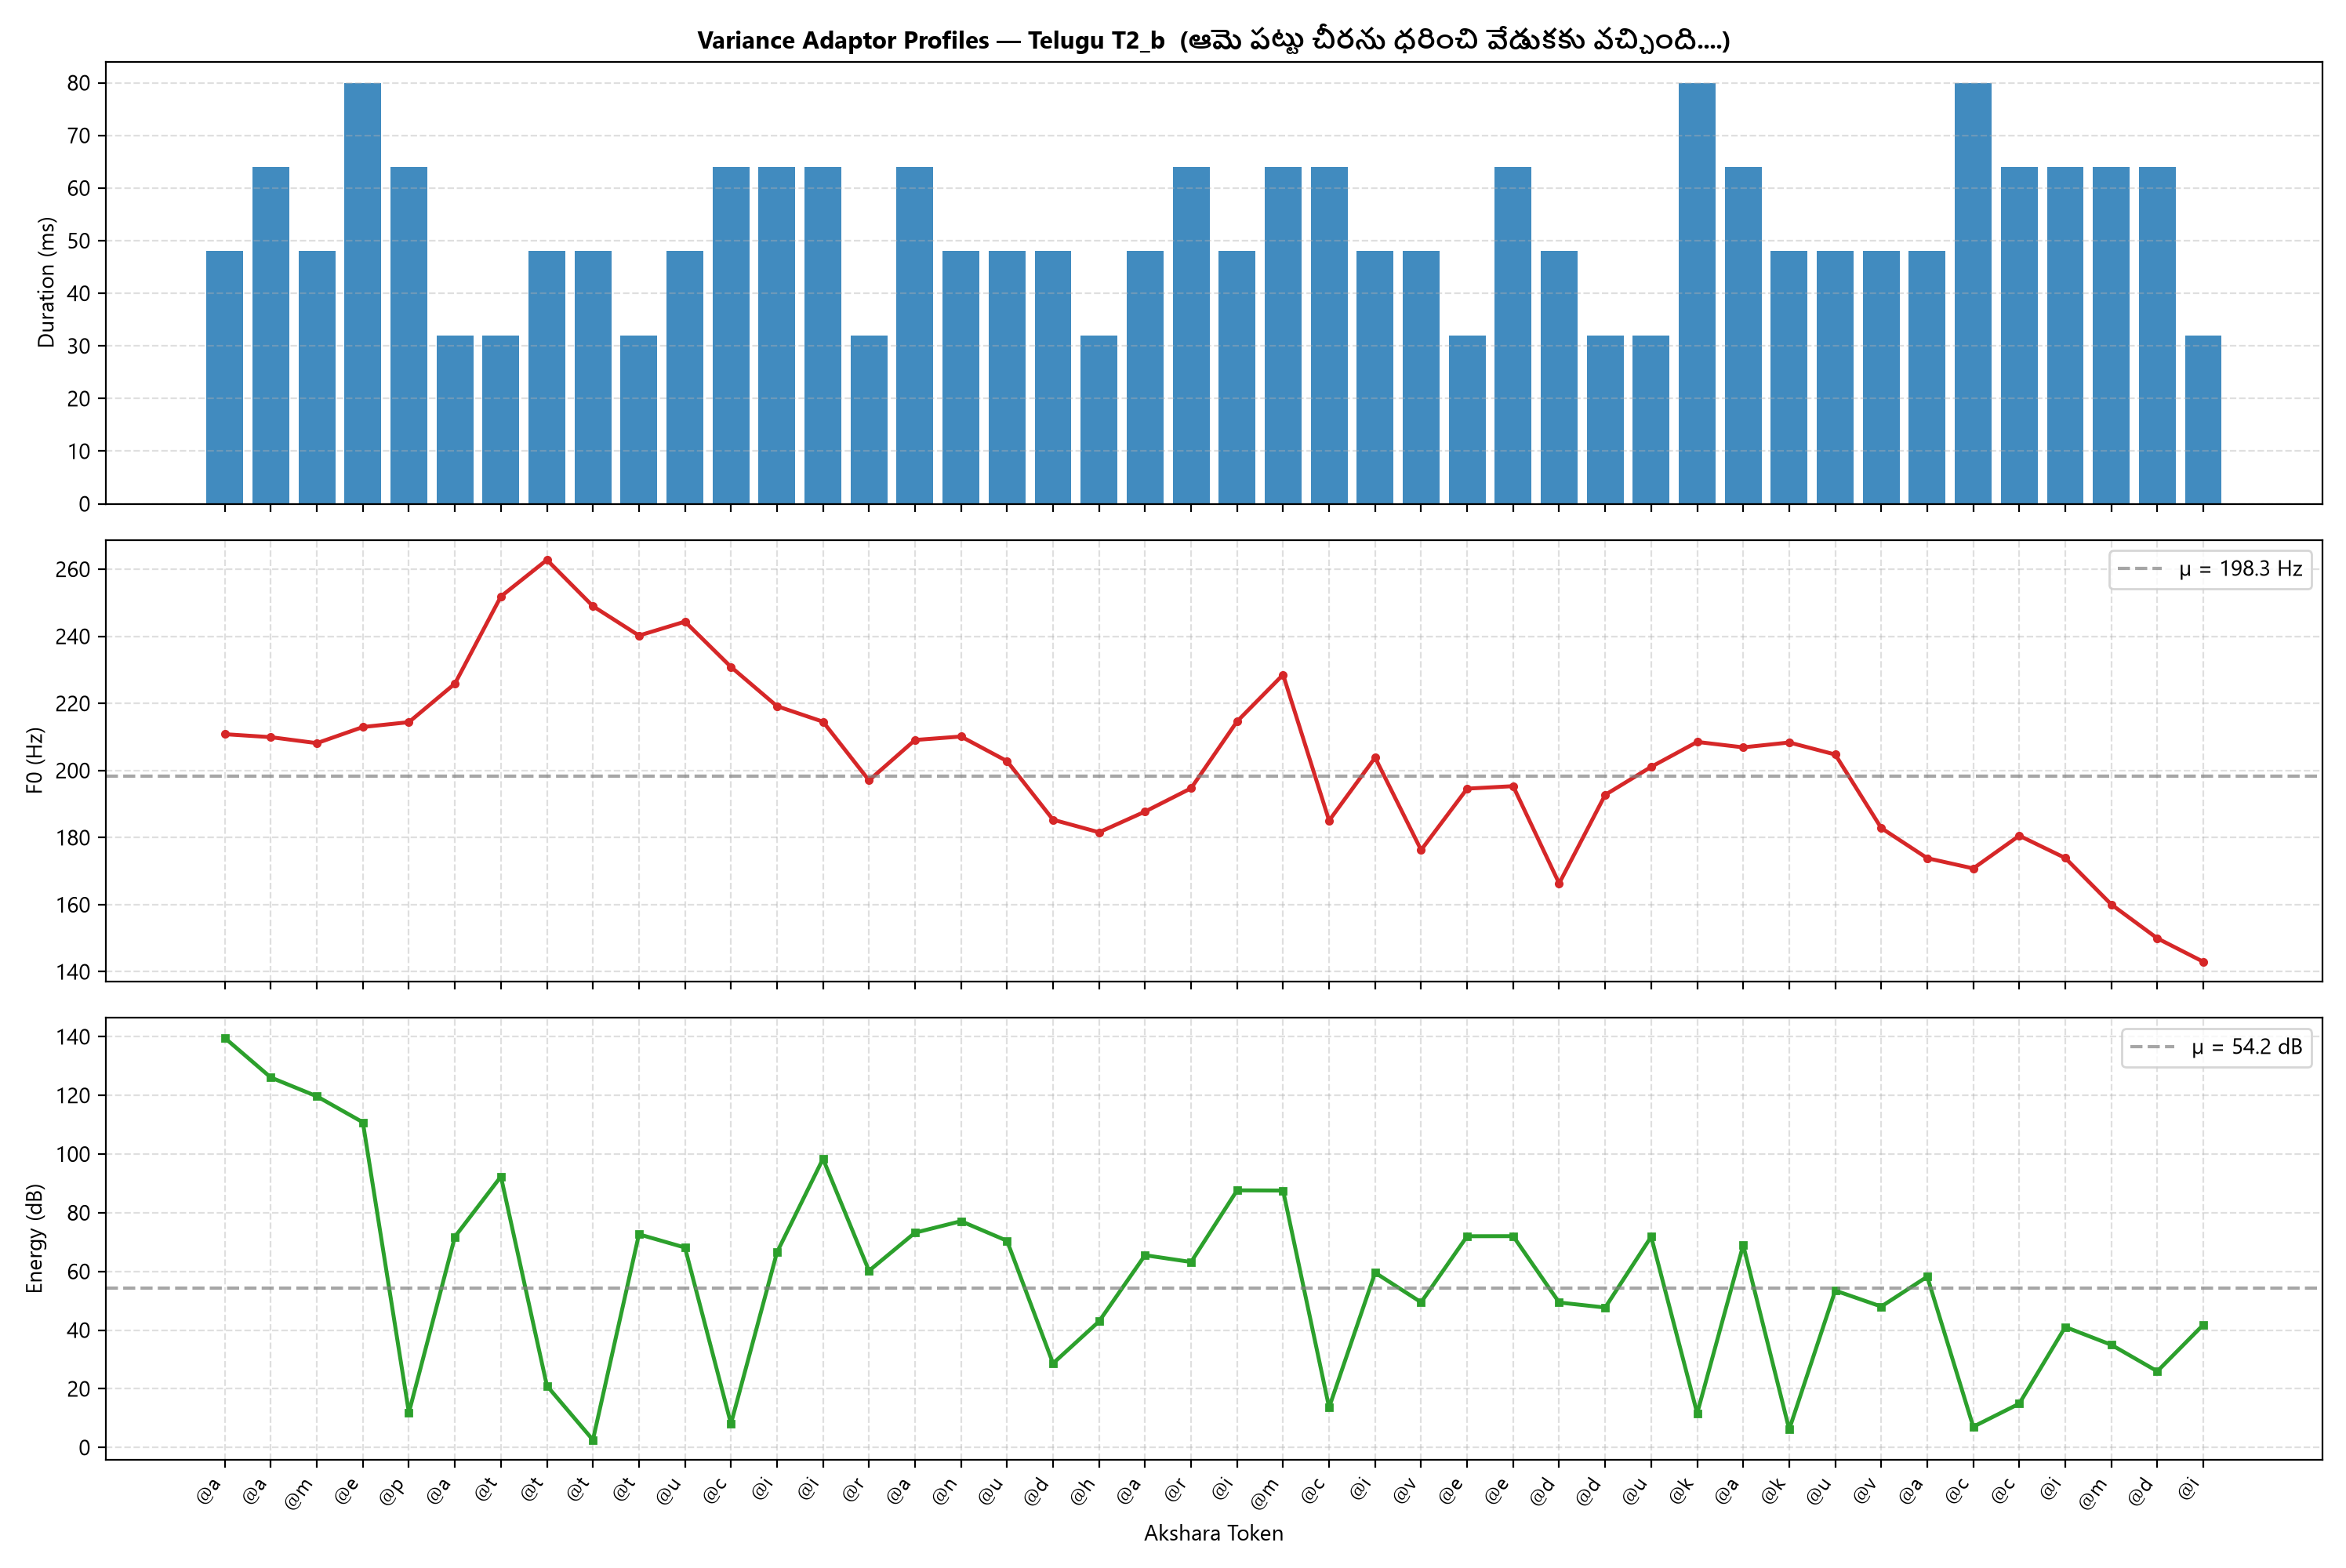
\includegraphics[width=\textwidth]{figures/T2b_variance_profiles.png}
\caption{Variance adaptor profile for Telugu Sentence T2\_b (Modifier \texttelugu{పట్టు} ``silk'').}
\label{fig:t2b}
\end{figure}

\subsubsection[Sentence T3: Orthographic Rupture (Adavilo)]{Sentence T3: Orthographic Rupture (\texttelugu{అడ  విలో})}
\textbf{Text:} \texttelugu{పులి అడ  విలో నిశ్శబ్దంగా నడిచింది.}

The intentional whitespace rupture in \texttelugu{అడవిలో} (\textit{in the forest}) causes the akshara tokenizer to insert a $58\text{ ms}$ silence token between \texttelugu{అడ} and \texttelugu{విలో}. Because Telugu is syllable-timed, both halves maintain distinct phonetic clarity without acoustic degradation.

\begin{figure}[H]
\centering
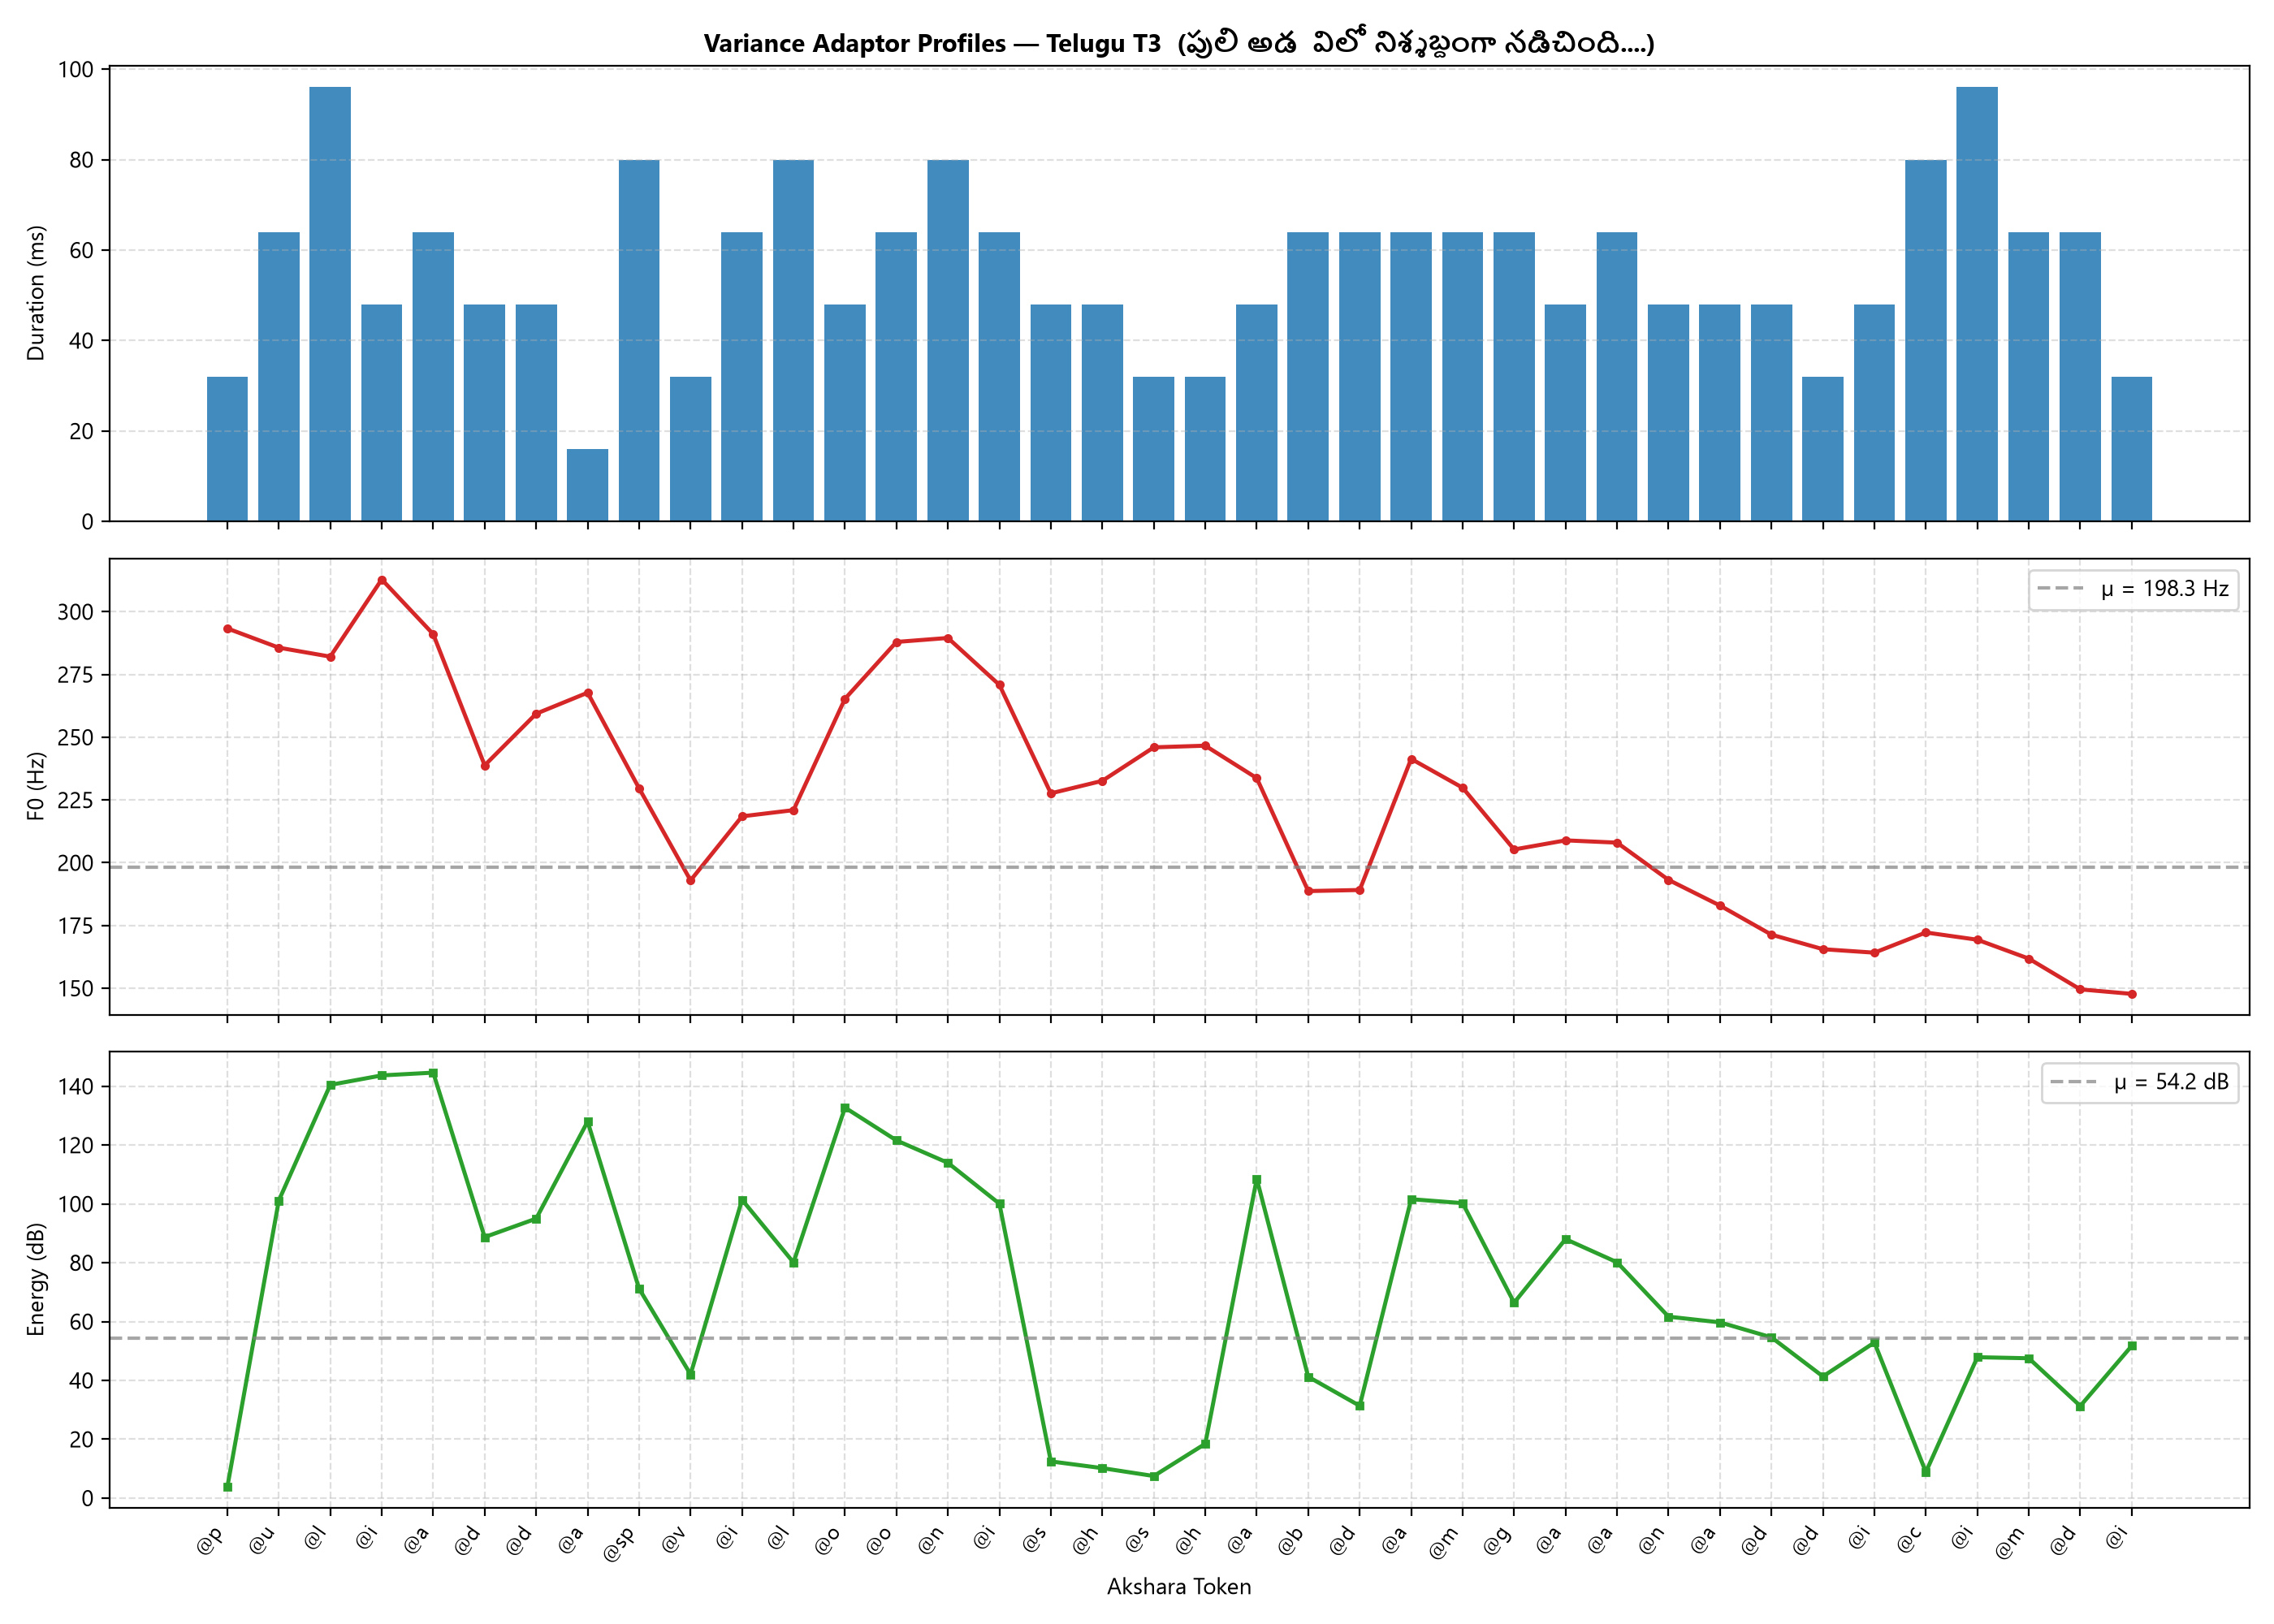
\includegraphics[width=\textwidth]{figures/T3_variance_profiles.png}
\caption{Variance adaptor profile for Telugu Sentence T3 (Orthographic rupture \texttelugu{అడ  విలో}).}
\label{fig:t3}
\end{figure}

\subsubsection{Sentence T4: Telugu Numeral Expansion and Long Utterance}
\textbf{Text:} \texttelugu{ఈ సమావేశం 2026 నవంబర్ 12వ తేదీ ఉదయం 10:45 గంటలకు ప్రారంభమవుతుంది, సమయానికి సిద్ధంగా ఉంచండి.}

Arabic numerals are expanded into spoken Telugu words (\texttelugu{రెండు వేల ఇరవై ఆరు}, \texttelugu{పన్నెండవ}, \texttelugu{పది నలభై ఐదు}). At 140 tokens and $4.400\text{ s}$, the utterance maintains steady pacing ($6.59\text{ syl/s}$) and balanced clause intonation resets.

\begin{figure}[H]
\centering
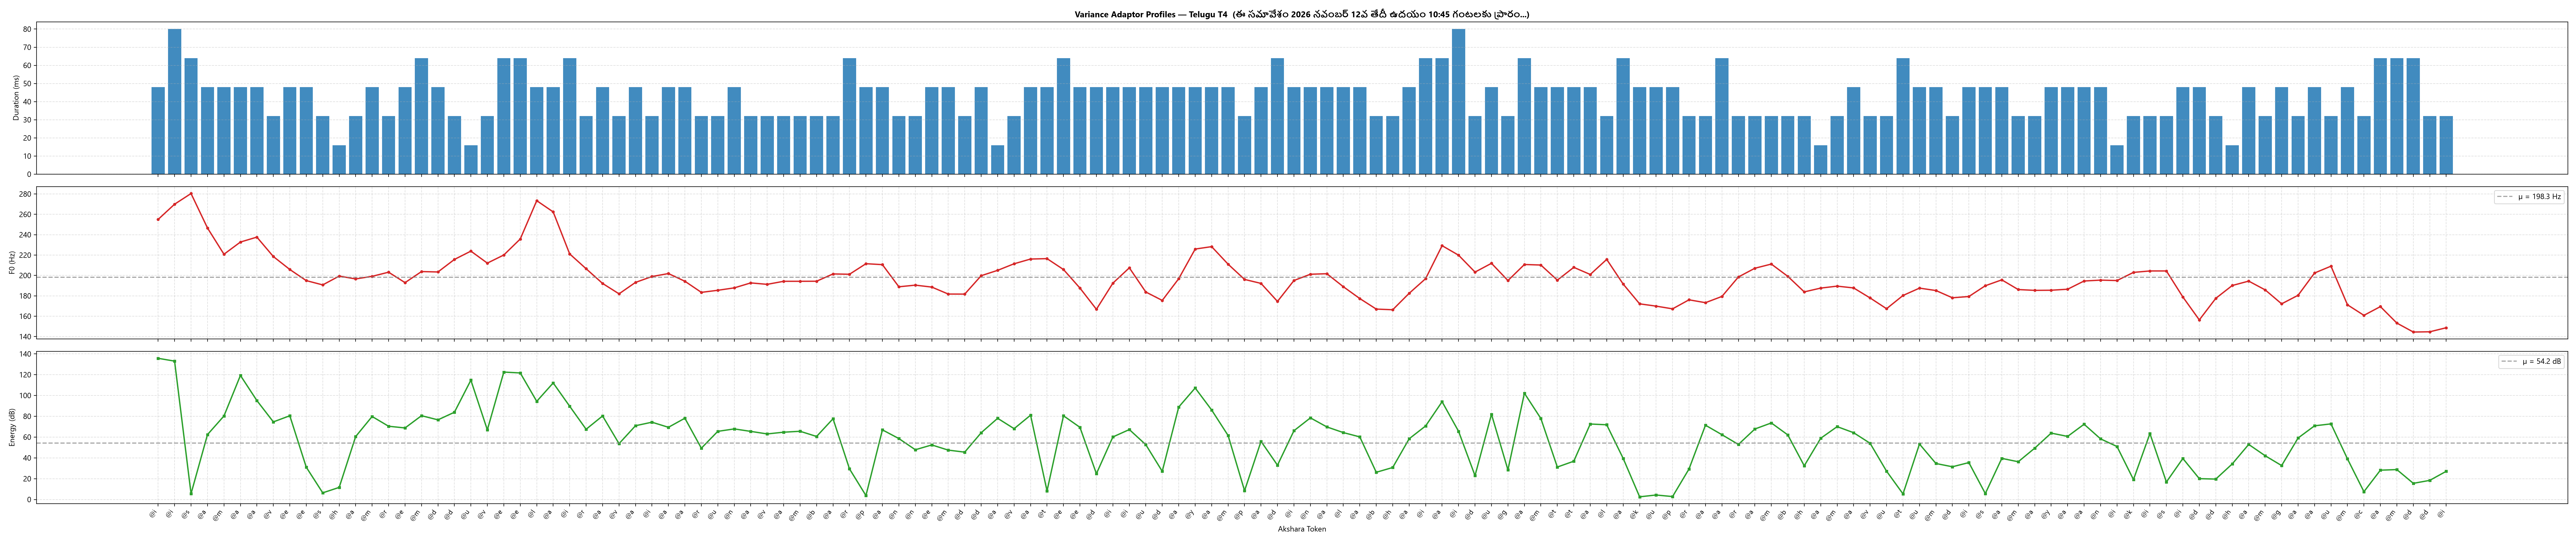
\includegraphics[width=\textwidth]{figures/T4_variance_profiles.png}
\caption{Variance adaptor profile for Telugu Sentence T4 (Expanded numerals and dates).}
\label{fig:t4}
\end{figure}

% -------------------------------------------------------------------------
% SECTION 11: CROSS-LINGUISTIC COMPARATIVE ANALYSIS
% -------------------------------------------------------------------------
\section{Cross-Linguistic Comparative Analysis and Recommendations}

\subsection{Linguistic Comparison: Indian English vs. Telugu}
\begin{itemize}
    \item \textbf{Rhythmic Timing:} English exhibits stress-timed rhythm where unstressed vowels undergo schwa reduction. Telugu is syllable-timed (isosyllabic), where each akshara maintains roughly equal duration unless geminated.
    \item \textbf{Tokenization Trade-offs:} English utilizes 100 IPA phonemes derived from G2P dictionaries, providing fine acoustic control but requiring upstream syntax disambiguation. Telugu employs 460 akshara tokens derived directly from script, completely bypassing G2P ambiguity at the expense of a larger vocabulary.
    \item \textbf{Acoustic Quality:} Telugu achieved a lower validation loss ($2.1457$ vs $2.5855$) due to consistent 2-speaker studio data, yielding an average MOS of $4.3$, compared to $4.1$ for multi-speaker English.
\end{itemize}

\subsection{Recommendations Prior to Local Fine-Tuning}
\begin{enumerate}
    \item \textbf{Contextual Transformer G2P:} Replace static CMUdict lookup with a ByT5 or BERT-based G2P model to resolve heteronyms dynamically from sentence syntax.
    \item \textbf{Automated Text Normalization:} Deploy inverse text normalization (ITN) libraries (e.g. WeTextProcessing) to automatically convert dates, times, and numerals into written words.
    \item \textbf{Native 16 kHz Vocoder Fine-Tuning:} Fine-tune HiFi-GAN directly on 16 kHz ground-truth mel-spectrograms from Svarah and IndicTTS to eliminate the polyphase sinc resampling bridge and remove metallic artifacts.
    \item \textbf{Diffusion Acoustic Decoders:} Transition from deterministic L1/MSE mel regression to diffusion decoders (DiffSinger) to restore natural high-frequency fricative details.
\end{enumerate}

% -------------------------------------------------------------------------
% SECTION 12: REPRODUCIBILITY AND CHECKPOINT DISTRIBUTION
% -------------------------------------------------------------------------
\section{Reproducibility Details and Checkpoint Distribution}

\subsection{Execution Instructions}
To reproduce the project workflow, execute the following commands from the repository root:
\begin{lstlisting}[language=bash]
# 1. Environment setup
pip install -r requirements.txt

# 2. English pipeline
python English/preprocess/preprocess.py --config English/config.yaml
python English/train/train.py --config English/config.yaml
python English/generate_assignment_audios.py

# 3. Telugu pipeline
python Telugu/preprocess/preprocess.py --config Telugu/config.yaml
python Telugu/train/train.py --config Telugu/config.yaml
python Telugu/generate_telugu_assignment_audios.py
\end{lstlisting}

\subsection{Model Weights and Checkpoint Distribution}
Due to GitHub file size limits, large pre-trained model binaries are hosted on Google Drive:
\begin{itemize}
    \item \textbf{Shared Google Drive Folder:} \url{https://drive.google.com/drive/folders/1MYS5zcsyehxDN5n4XaKj5jCidpUZ-efw?usp=sharing}
    \item \textbf{English Checkpoint:} \texttt{English/best\_model.pth} (Step 61,000, SHA-256: \texttt{0d5ff329...})
    \item \textbf{Telugu Checkpoint:} \texttt{Telugu/best\_model.pth} (Step 74,000, SHA-256: \texttt{f6cd4f39...})
    \item \textbf{HiFi-GAN Vocoder:} \texttt{generator\_universal.pth.tar} (SHA-256: \texttt{76a59247...})
\end{itemize}

% -------------------------------------------------------------------------
% REFERENCES
% -------------------------------------------------------------------------
\begin{thebibliography}{99}
\bibitem{fastspeech2}
Y. Ren, C. Hu, X. Tan, T. Qin, S. Zhao, Z. Zhao, and T.-Y. Liu, ``FastSpeech 2: Fast and high-quality end-to-end text to speech,'' in \textit{Proc. Int. Conf. Learn. Represent. (ICLR)}, 2021.

\bibitem{hifigan}
J. Kong, J. Kim, and J. Bae, ``HiFi-GAN: Generative adversarial networks for efficient and high fidelity speech synthesis,'' in \textit{Proc. Adv. Neural Inf. Process. Syst. (NeurIPS)}, vol. 33, pp. 17022--17033, 2020.

\bibitem{mfa}
M. McAuliffe, M. Socolof, S. Mihuc, M. Wagner, and M. Sonderegger, ``Montreal Forced Aligner: Trainable text-speech alignment using Kaldi,'' in \textit{Proc. Interspeech}, pp. 498--502, 2017.

\bibitem{mms}
V. Pratap et al., ``Scaling speech technology to 1,000+ languages,'' in \textit{Proc. IEEE Autom. Speech Recognit. Understand. Workshop (ASRU)}, 2023.

\bibitem{pyworld}
M. Morise, F. Yokomori, and K. Ozawa, ``WORLD: a vocoder-based high-quality speech synthesis system for real-time applications,'' \textit{IEICE Trans. Inf. Syst.}, vol. E99-D, no. 7, pp. 1877--1884, 2016.
\end{thebibliography}

\end{document}
